%%%%%%%% ICML 2021 EXAMPLE LATEX SUBMISSION FILE %%%%%%%%%%%%%%%%%

\documentclass{article}

% Recommended, but optional, packages for figures and better typesetting:
\usepackage{microtype}
\usepackage{graphicx}
\usepackage{subfigure}
\usepackage{booktabs} % for professional tables
\usepackage{amsmath}
\usepackage{amsfonts}
\usepackage[shortlabels]{enumitem}


% hyperref makes hyperlinks in the resulting PDF.
% If your build breaks (sometimes temporarily if a hyperlink spans a page)
% please comment out the following usepackage line and replace
% \usepackage{icml2021} with \usepackage[nohyperref]{icml2021} above.
\usepackage{hyperref}

% Attempt to make hyperref and algorithmic work together better:
\newcommand{\theHalgorithm}{\arabic{algorithm}}

% Use the following line for the initial blind version submitted for review:
% \usepackage{icml2021}

% If accepted, instead use the following line for the camera-ready submission:
\usepackage[accepted]{icml2021}

% The \icmltitle you define below is probably too long as a header.
% Therefore, a short form for the running title is supplied here:
\icmltitlerunning{A Survey of Graph Neural Networks for Programming Languages}

\begin{document}

\twocolumn[
\icmltitle{A Survey of Graph Neural Networks for Programming Languages}

% It is OKAY to include author information, even for blind
% submissions: the style file will automatically remove it for you
% unless you've provided the [accepted] option to the icml2021
% package.

% List of affiliations: The first argument should be a (short)
% identifier you will use later to specify author affiliations
% Academic affiliations should list Department, University, City, Region, Country
% Industry affiliations should list Company, City, Region, Country

% You can specify symbols, otherwise they are numbered in order.
% Ideally, you should not use this facility. Affiliations will be numbered
% in order of appearance and this is the preferred way.
\icmlsetsymbol{equal}{*}

\begin{icmlauthorlist}
\icmlauthor{Hemil Desai}{equal,ucla}
\icmlauthor{Sripath Mishra}{equal,ucla}
\icmlauthor{Justin Yi}{equal,ucla}
\end{icmlauthorlist}

\icmlaffiliation{ucla}{Department of Computer Science, University of California, Los Angeles}

\icmlcorrespondingauthor{Hemil Desai}{hemil10@ucla.edu}
\icmlcorrespondingauthor{Sripath Mishra}{mishra60@ucla.edu}
\icmlcorrespondingauthor{Justin Yi}{joostinyi00@gmail.com}

% You may provide any keywords that you
% find helpful for describing your paper; these are used to populate
% the "keywords" metadata in the PDF but will not be shown in the document
\icmlkeywords{Machine Learning, ICML}

\vskip 0.3in
]

% this must go after the closing bracket ] following \twocolumn[ ...

% This command actually creates the footnote in the first column
% listing the affiliations and the copyright notice.
% The command takes one argument, which is text to display at the start of the footnote.
% The \icmlEqualContribution command is standard text for equal contribution.
% Remove it (just {}) if you do not need this facility.

% \printAffiliationsAndNotice{}  % leave blank if no need to mention equal contribution
\printAffiliationsAndNotice{\icmlEqualContribution} % otherwise use the standard text.

\begin{abstract}
This document provides a basic paper template and submission guidelines.
Abstracts must be a single paragraph, ideally between 4--6 sentences long.
Gross violations will trigger corrections at the camera-ready phase.
\end{abstract}

\section{Decompilation}
\label{decompilation}

\subsection{Introduction}
Compiled languages are languages whose source code is compiled into machine understandable code by compilers. This machine code can directly be read and executed by the processor. This low-level machine code can either be in binary form or some other intermediate form. Due to the compilation process, these languages are generally faster and more efficient in addition to giving fine-grained control over hardware variables like memory, CPU and GPU, etc. Most popular compiled languages include Java, C, C++, Go, Rust, etc. The process of converting high level source code into low level machine code or other intermediate formats is called Compilation. This is achieved by compilers and is pretty straight forward once we have access to the language specific compiler.

Naturally, the inverse process involves taking machine code in binary format and retrieving the source code. This inverse process is called Decompilation. This process is not so trivial and involves many complex challenges. The semantics of the high level programming language are often lost during compilation. \citet{coda} state that there are both intra-statement and inter-statement dependencies in the low-level instructions that need to be preserved by the decompiler. Although challenging, Decompilation is necessary in a variety of applications. Security analysis is crucial for low level code, and decompilation can help in areas like malware analysis and vulnerable software patching as presented in \citet{kolbitsch2009effective} and \citet{yakdan2016helping}. Moreover, \citet{lee2011tie} show that malicious attackers can use decompilers to reverse engineer low level code and exploit commercial software. \citet{katz2019towards} also mention that decompilation can be useful for porting code to different hardware as well as source level analysis and optimization tools. Hence, having efficient and accurate decompilation tools can be of utmost importance.

\subsection{Conventional Decompilers}
Lots of research have been done for Decompilers over the years \cite{cifuentes1994reverse, emmerik2004using,brumley2011bap,bao2014byteweight,rosenblum2008learning,yakdan2016helping,brumley2013native}. Many rule-based and pattern matching decompilers have been developed like Hex-Rays \cite{hexray}, Phoenix \cite{brumley2013native} and the most recent one RetDec \cite{kvroustek2017retdec}. These compilers use pre-defined rules to match patterns in the low level code to control flow graphs of the high level code and translate the instructions accordingly. When such patterns are not found, the decompiler uses \textit{goto} statements in C. This is just like a line-to-line translation from low level code to C. Some decompilers like DREAM++ \cite{yakdan2015no,yakdan2016helping} exist which do not use \textit{goto} statements. However, these are still hand crafted.

Such hand-crafted compilers face a variety of problems like:
\begin{itemize}
    \item Most of these decompilers are handcrafted for a specific source-target language pair. This requires a lot of effort in itself, and this effort has to be replicated for each new source-target pair for which we want to build a decompiler.
    \item The output high level code fails to preserve the functionality of the low level code in most cases.
    \item The output high level code is not semantically readable and often lacks human friendliness. It also fails to use abstractions to represent the high level code as humans do. As a result, the reversed code is often hard to interpret and use it in corresponding applications.
\end{itemize}

\subsection{Problem Definition}
\citet{coda} gives a nice technical definition of the problem which we can reuse here. Let $P$ denote the high level program and $\tau$ denote the compiler. Hence, we can get the low level code as $\phi = \tau(P)$. They define the decompiler $\tau^{-1}$ that satisfies $\tau(P^{'}) = \tau(P) \text{ where } P^{'} = \tau^{-1}(\phi)$.

\subsection{Data Generation}
Data generation for decompilation tasks is relatively trivial due to the free availability of compilers. However, there are still some challenges. Generating source-target pairs can be done by taking the source code and running it through a compiler to get the executable or low level code. Nuances involve selecting the source code, selecting the different architectures for the compiler, selecting whether to produce the executable or the assembly instructions, etc. 

\citet{katz2018using} suggest creating a database of source-target pairs by compiling programs using a customized compiler based on Clang and LLVM. This compiler pairs AST trees and subtrees of source code with the corresponding low level machine code output by the compiler.They constrain the pairs by adding the following restrictions - 112 or fewer binary low level tokens and 88 or fewer source code tokens. The programs they use for their dataset are from open source RPMs for Fedora containing C source code. Comprehensive details are provided in their paper.

\citet{katz2019towards} generate samples for their decompiler to train on using random code samples from a subset of the C programming language. They do this by sampling the grammar of the language. These samples are guaranteed to be syntactically and grammatically correct. They then compile their code samples using the provided compiler. Doing so results in a dataset of matching pairs of statement, one in C and the other in Lll , that can be used by the model for training and validation. Note the two differing approaches here - taking C code from open source repos vs. using sampling to generate C source code. 

\citet{coda} use a two-step approach to decompilation (which we will discuss later). To build the dataset for stage 1, they randomly generate 50,000 pairs of high level programs with their corresponding compiled low level code. The compilation occurs using clang with all optimizations disabled. The source code programs can be roughly classified into short and long programs with an average length of 15 and 30 each. Their corresponding tree representations have a maximum depth of 3. They also use real world programs like neural network construction programs in pytorch C++ API and Hacker’s Delight loop-free programs. The dataset for the next stage is constructed by injecting various types of errors into the high level program. 10-20\% token errors are injected. The locations for these errors are sampled randomly using a uniform distribution. Once again, detailed statistics and methods are provided in their paper.

N-Bref \cite{nbref} assess the performance of their model on various benchmarks by using both generated high level code using their dataset generator as well as code written by humans in the form of Leetcode solutions to Problems (2017). The binary low level code is assembled using the GNU binary utilities to obtain the assembly code. To generate ASTs for the high level C code, the authors implement a parser using clang compiler for python. Their dataset generator for generated samples is built on top of csmith \cite{yang2011finding} - a code generation tool for compiler debugging. Their dataset generator avoids expression collision (EC). For instance, unary operators like \textit{i++} are converted to binary operators like \textit{i = i + 1} and all while loops are converted to for loops. This improves performance and also reduces confusion. The dataset generator also has several hyperparameters to control the depth, size, nesting, etc of the high level code. Here also the code is compiled with no optimizations. Previous works \cite{brumley2013native,lee2011tie,lin2010automatic} also
disabled optimizations, because many optimizations change variable types and rewrite source code
(e.g. loop-invariant optimization) which will result in unfair accuracy evaluations. Their dataset is available to download from \url{https://www.dropbox.com/s/33fop57jjq0wwa9/POJ-104.tar.gz?dl=1}.

A common theme across approaches is to take high level source code (mostly in C) and use compilers with some flags to generate the corresponding dataset pairs. Each approach tunes some nuances to generate their own datasets, but at the high level they have a lot of similarities. For future research, it will be nice to have a common benchmark and dataset for decompilation tasks. A common benchmark will aid in unbiased comparison of different methods and will also help more people easily research novel methods once a common dataset is easily available.

\subsection{Evaluation}
There are many different ways to evaluate decompilation tasks. You could compare the difference between the original source code and the generated source code using something like Levenshtein edit distance (LD) \cite{hyyro2001explaining}. You could compare the output of the original source code and the generated source code by compiling and then executing the binaries. Other works use BLEU, edit distance ratio, and syntactic correctness ratio \cite{nguyen2013lexical}. We will take a look at some of the approaches used by papers that use neural methods for decompilation.

\citet{katz2018using} use a separate test dataset to evaluate their model. They feed their trained model sequences of binary input code. The model outputs a series of tokens corresponding to the predicted output in the source language C aka the generated C source code. They use two evaluation metrics to assess the quality of the C source code generated by their technique. Since they use RNNs, the first metric, perplexity, is based on the RNN’s internal sampled softmax loss function, as described in \citet{jean2014using}, and is used during RNN training. It is a measure of the accuracy of a probabilistic model in predicting a sample \cite{shannon2001mathematical}. They use the perplexity measurement as a proxy for RNN performance to determine when to end training. The second metric is
based on the Levenshtein edit distance between the sequence of tokens in the ground truth source code associated with a given binary sequence and the sequence of tokens output by the RNN. They use two variations on edit distance. First is to look at straight edit distance between the tokens in the prediction and those in the ground truth snippet. Second, to ensure differences in identifier names and constants do not influence results, they lex both the output translations and ground truth snippets to obtain sequences of token types and perform the edit distance calculation between corresponding sequences of token types. They report the average edit distance for the exact tokens predicted; the average edit distance for the types of tokens predicted; and the percent of predicted token sequences that match the ground truth token sequences perfectly, without post-processing.

On the other hand, \citet{katz2019towards} uses the deterministic nature of the compiler to evaluate their model. After translating the inputs, for each pair of input i and corresponding translation t (i.e. the decompiled code), they recompile t and compare the output to i. This allows them to keep track of progress and success rates, even when the correct translation is not known in advance. Exact details are described in the paper. Despite holding the ground-truth for the test set (the C used to generate the set), they decided not to compare the decompiled code to the ground-truth because in some cases, different C statements could be compiled to the same low-level code (e.g. the statements x = x + 1 and x++). They believe that their evaluation method allows for such occurrences and is closer to what would be applied in a real use-case.

\citet{coda} (Coda) assess the performance of their model on various synthetic benchmarks with different difficulty levels and real-world applications. Given the binary executable as the input, we use an open-source disassembler \cite{mips,redasm} for MIPS \cite{hennessy1982mips} and x86-64 \cite{guide2011intel} architecture to generate the corresponding assembly code that is fed to the model. They evaluate the performance of the Coda using two main metrics: token accuracy and program accuracy. Token accuracy is defined as the percentage of the predicted tokens in high-level Programming Language that match with the ground-truth ones. Program accuracy is defined as the ratio between the number of predicted programs with 100% token accuracy and the number of total recovered programs.

\cite{nbref} uses different metrics for different stages of their model. For the source code generation stage, they use token accuracy and the graph edit distance \cite{sanfeliu1983distance} without enforcing the match between predicted and ground truth AST on graph generation. The metric is fair to evaluate decompilation tasks as we remove all the Expression collision. For the data-type solver stage, they use two metrics: (i) macro accuracy and (ii) micro accuracy.

Often, these metrics are combined and calculated in ways that give the success rates of decompilation in percentages. The evaluation metrics and protocol seem to vary across different neural decompilation approaches. This makes consistent evaluation across different methods difficult. Since this is a fairly recent research area, a standard evaluation benchmark and metric along with the standard dataset proposed earlier will aid in moving research forward in this domain.

Next we will discuss the different neural decompilation approaches at a high level.

\subsection{RNN and Neural Machine Translation (NMT) based approaches}
RNNs have become very popular for sequential Machine Learning tasks like translation, question answering ,etc \cite{sutskever2014sequence}. RNNs have feedback loops which permit persistence of data which in turn allows sequential processing \cite{siegelmann1993foundations}. An unrolled recurrent neural network has a natural sequence-like structure which makes it well suited for translation tasks. There are several variations on RNNs including the LSTM \cite{hochreiter1997long} which has increasingly become the go-to RNN of choice. LSTMs help preserve long term dependencies and have shown major improvements when dealing with longer sequences. A particular variant of RNNs is the sequence to sequence model or the seq2seq, which takes in an input sequence and generates an output sequence. As you can imaging, such seq2seq models are very useful for tasks like natural language translation \cite{cho2014learning}.

Decompilation can be seen as a natural expansion of the language translation task, but for programming languages. Translation for programming languages can also include translating between two high level languages like Java and Python. But decompilation deals with translation between a high level language and a low level binary executable/machine code. 

\citet{katz2018using} is one of the first approaches to adapt seq2seq RNN models for decompilation. Their sequence-to-sequence model is composed of two recurrent neural networks: an encoder, which processes the input sequence, and a decoder,
which creates outputs. Further, the sequence-to-sequence model contains a hidden state, C, which summarizes the entire input sequence. The output is generated from the decoder by taking in the hidden state and the current input and yielding a probability distribution from an activation function like Softmax. To modify this model for decompilation, they make many changes in all steps of the pipeline including pre-processing, model architecture, post-processing, etc. The first step involves tokenization of the input-output pair i.e. the source-target pair of the high level code/ low level code pair. The appropriate tokenizer is chosen and built based on expert domain knowledge. The authors also use bucketing to separate out different lengths of the input sequence \cite{bucketing}. Each bucket has its own RNN comprising of the encoder and decoder. Exact details can be found in the paper. The pipeline for an input pair looks like this - 
\begin{itemize}
    \item The binary low level code is tokenized and converted to a list of integers corresponding to the indices in the dictionary for the low level code of the tokenizer.
    \item The list of integers goes through bucketing to choose the relevant bucket and RNN
    \item The list then goes through the encoder to generate a hidden state for the binary code.
    \item The decoder then takes this state and outputs a probability distribution representing tokens in the high level code. This distribution is then converted to a list of integers with the integers corresponding to the indices in the dictionary for the high level code in the tokenizer.
    \item The tokens for the high level code are retrieved and combined from that dictionary.
\end{itemize}

This approach does not take into consideration the differences between natural languages and programming languages, thus leading to ineffective results. For example, as \citet{katz2019towards} point out, the code they generate often cannot be compiled or is not equivalent to the original source code. This approach did however show the possibility of NMT for decompilation, and served as a stepping stone for the next approach proposed by \citet{katz2019towards}. 

\citet{katz2019towards} combines Neural Machine Translation (NMT) and Program analysis to improve the performance of their Neural Decompilation model and make it more practically useful and viable. They also propose a framework called TraFix that can automatically learn a decompiler from a compiler and check the correctness of the decompiler using a verifier. Their approach consists of two complimentary phases:
\begin{itemize}
    \item Generating a code template that, when compiled, matches the computation structure of
the input. The input is the low level binary code.
    \item Filling the template with values and constants that result in code equivalent to the input. This means that the output from running the executable will be the same for both cases.
\end{itemize}
They use a NMT model combined with a feedback loop which facilitates active learning based on the outputs of phase 1. Phase 1 results are compared to the computation structure of the input. If they match, the generated code moves to phase 2. If not, the dataset is updated and the model is trained again. The authors use LSTMs for their NMT model.

NMT based techniques are still primarily sequential and fail to incorporate the graph and tree structures of code like control flow graphs and abstract syntax trees. We will take a look at some newer methods which try to incorporate these properties.

\subsection{Abstract Syntax Tree (AST) based Neural Decompilation}
Coda \cite{coda} also uses a two phase learning approach and an NMT model at its base. But it tries to incorporate the code structure into the encoder and decoder of the RNN. Its two phase approach can be described as:
\begin{itemize}
    \item It uses an instruction type-aware encoder and a abstract syntax tree (AST) decoder
for translating the input binary into the target PL. Their encoder deploys separate RNNs for different
types of statements, thus the statement boundaries are preserved (This is different from bucketing used by \citet{katz2019towards}. Furthermore, the control and data dependency in the input program are translated to the connections between the hidden states of corresponding RNNs. The output from the AST decoder maintains the dependency constraints and statement boundaries using terminal nodes, which facilitates learning the grammar of the target PL.
    
    \item In this stage, Coda employs an RNN-based error predictor (EP) to identify potential
prediction mistakes in the output program from Phase 1. Ensembling method can be used to boost
the performance of the error prediction. The EP is used to guide the iterative correction of the output
program. Unlike traditional decompilers which utilize only the syntax information from the input,
Coda leverages the Levenshtein edit distance (LD) between the compilation of the updated output
program and the ground-truth low-level code to prevent false alarms induced by the EP. This can be considered conceptually similar to phase 2 of \citet{katz2019towards}.

They also employ a technique called Attention Feeding to combine different contexts in the AST decoder. This can be considered similar to message passing in graphs, since trees are a form of graph. The Attention Feeding is comprised of parent attention feeding and input instruction attention feeding. Parent feeding refers to context from the parent of the current node, and input feeding refers to context from the current node's corresponding node in the input.
\end{itemize}

\subsection{Bringing Graph Neural Networks into the picture}
Even after incorporating AST structure, the base models of the previous approach are still derived from natural language based seq2seq models. This disregards the intrinsic structure of code (graphs/trees). To the best of our knowledge, \cite{nbref} is the first Neural Decompilation approach which utilizes Graph Neural Networks (GNNs) to represent code in the context of decompilation. They use a backbone structural transformer \cite{vaswani2017attention} with inductive Graph Neural Networks \cite{hamilton2017inductive} to represent the low-level code (LLC) as control/dataflow dependency graphs and source code as Abstract Syntax Tree (AST).

Their pipeline also involves a two step approach - data type solver (DT-Solver) and source code generator (SC-Gen). The output of the data type solver is used as the decoder input of the source
code generation. Both use the same backbone with GNNs.

\textbf{Structural Transformer with GNNs}
The backbone structural transformer has three components: (1) LLC encoder, (2) AST encoder, and (3) AST decoder. The LLC encoder takes the low-level instructions converted from binaries using disassembler as input. AST encoder takes the input of a previous (partial) AST, and the predictions of AST decoder are AST nodes, which can be equivalently converted to the high-level program. Here we will focus on the encoders and how they use GNNs. The GNN of choice in this paper is GraphSAGE (\citet{hamilton2017inductive}). GNNs are used in two places - 1) To embed the initial code/AST structure 2) To augment the Attention Layers in the Transformer



\textbf{Initial GNN embeddings}
The LLC encoder converts the initial low level code into a graph where each node is representated by its feature vector including features like register / instruction type ($var_t$
/ $ins_t$), position in the instruction ($n_{pos}$), node id ($n_{id}$) and numerical field ($n_{num}$). Edges are generated using hand crafted rules. Aggregation is done using max pooling. Aggregation vector and current state of the node are fed into a fully connected layer to get the next state. 3 layers are used for the GNN.

The AST encoder encodes the AST tree from the AST decoder to guide future
tree expansions. They treat the AST tree as a graph (V) and embed it using GraphSAGE as well. The input of the GNN includes meta-features of the tokenized AST node and a boolean indicating whether the node is expanded in this step. The output hidden states from the GNN is fed into the self-attention module. At the end of the AST encoder, they integrate the AST encoder output and LLC encoder output using an additional multi-head attention layer.


\textbf{GNN Augmentation for Attention}
The output of the attention layers is converted to a graph using the same edge rules in the LLC encoder and those states are then fed again into the GNN to obtain embeddings that incorporate the inductive biases of GNNs.

Experiments show that Nbref outperforms the corresponding transformer baseline and previous Neural Decompilers like Coda \cite{coda}. It also outperforms other models on human written Leetcode solutions. The performance gain over baseline Transformer clearly shows the value of using GNNs. Since most state of the art NMT models use transformers now, performance gains over previous Neural Decompilers using RNNs is expected. 

Critics for Nbref have mentioned that they do not propose anything novel, but the use of GNN based representations in Neural Decompilation is definitely the first we have come across. GNNs to represent code is a natural choice in many domains related to programming languages because of the graph and tree based structure of code. We believe future research will definitely involve the use of GNNs for learning representations of code. The way this is done might be tailored differently for decompilation to improve performance and efficiency. Once again, a common dataset and benchmark may help accelerate research in Neural Decompilation. 

\section{CodeXGlue}
Benchmarks in Natural Language Processing have played an important role in the progress of the field. Particularly, GLUE \cite{wang2018glue} is a comprehensive benchmark for training, evaluating and analyzing natural language understanding systems. It includes 9 tasks with corresponding datasets and evaluation guidelines, a diagnostic dataset to analyze NLP systems and a public leaderboard to track progress in the field. As expected, Deep Learning systems have dominated the benchmark and even surpassed human performance. As a result of this, SuperGLUE \cite{wang2019superglue} has been released as a continuation of GLUE with harder challenges in order to further progress the field.

Benchmarks provide a unified and system agnostic way for several different researchers to compare their approaches on a common ground. Most NLP papers dealing with finetuning language models will mention GLUE or SuperGLUE, and publish their results to the public leaderboard \footnote{https://gluebenchmark.com/leaderboard}. Looking at the incredible success of such benchmarks in NLP warrants a similar benchmark in applying Machine Learning to the domain of Programming Languages and Code. That is precisely what the recently released CodeXGlue (\citet{lu2021codexglue}) aims to achieve. Similar to GLUE, CodeXGlue contains a bunch of tasks paired with their corresponding processed datasets and a public leaderboard. The leaderboard can be found at \url{https://microsoft.github.io/CodeXGLUE/} and the github repo is at \url{https://github.com/microsoft/CodeXGLUE}.

We have so far discussed many domains of Programming Languages across which Deep Learning and Graph Neural Networks have shown tremendous potential. Now, we intend to cover this benchmark as a unifying evaluation point that will guide further research in applying Deep Learning and GNNs to the domain of programming languages. We will cover the tasks of the benchmark in brevity and also include short descriptions of the baselines. We will end this section by looking at how Graph Neural Networks can be utilized to vastly improve scores across all tasks in the benchmark. We hope this will serve as viable research direction for interested people.

\subsection{Tasks}
CodeXGlue includes 14 datasets for 10 diversified code intelligence tasks covering the following scenarios:
\begin{itemize}
    \item code-code (clone detection, defect detection, cloze test, code completion, code repair, and code-to-code translation)
    \item text-code (natural language code search, text-to-code generation)
    \item code-text (code summarization)
    \item text-text (documentation translation)
\end{itemize}

The tasks can be summarized in Fig. ....... which is taken from their github repo. The last category of tasks \textit{text-text} leans more towards NLP but the rest contain code as their prime or major component. With code comes the intrinsic structure of programming languages including trees and graphs, and this varies greatly from natural languages. Therefore, we believe the inductive biases of Graph Neural Networks are very well suited to represent the code aspect in these tasks. Since this is a fairly recent benchmark, the leaderboard mostly contains baselines as of now. Most of the baselines mentioned in the CodeXGlue paper and papers like CodeBERT \cite{feng2020codebert} use transformer models which are directly adapted from their NLP counterparts. Hence, there is plenty of room for innovation and climbing the leaderboard on this benchmark. We will briefly cover the baselines and then see how Graph Neural Networks can be used to bolster these deep learning models.

\subsection{Baselines}
The baselines use different variants of Transformers as their backbone. The tasks can be approximately classified into understanding tasks like code search, code clone detection, defect detection, cloze test (similar to masked language modeling) and generative tasks like code repair, code translation, code completion, code generation, etc.

For code understanding tasks, the authors provide CodeBERT \cite{feng2020codebert} as a baseline. CodeBERT is very similar to BERT \cite{devlin2018bert} and treats programming language as sequential. The model is pretrained on the CodeSearchNet dataset \cite{husain2019codesearchnet} using a masked language modeling objective like BERT and a combination of comments and code as input. It is then fine tuned on the downstream CodeXGlue tasks.

For generative tasks like code generation and code completion, the authors provide CodeGPT as the baseline. CodeGPT is inspired from GPT2 \cite{radford2019better}. CodeGPT contains pre-trained monolingual models on Python and Java corpora from the CodeSearchNet dataset, which includes 1.1M Python functions and 1.6M Java methods. They provide two variants of this baseline, one trained from scratch and one using GPT2 as the starting point.

For tasks which are more seq2seq in nature like code translation, the authors provide a encoder-decoder baseline with CodeBERT as the encoder and a custom transformer as the decoder.

\subsection{Graph Neural Networks}
The baselines include models adapted from the NLP domain. As a result, the baselines treat code as natural language and disregards its intrinsic structure and syntactic biases. As we have seen throughout the paper, Graph Neural Networks have shown great promise in tasks related to programming languages. In section 1....... we saw the latest research in representing code using graph neural networks. In the rest of the sections, we saw how GNNs and representations using GNNs are adapted to specific domains. 

A lot of those techniques can be used across multiple tasks in CodeXGlue and we believe they can give consistent improvements as compared to the baselines. We will explore some ways that we envision GNNs being used across tasks in CodeXGlue.

\section{Program Similarity and Classification}
\label{similarity}
\subsection{Introduction}

Graph similarity search is one of the most important graph-based applications, with extensive applications to complex graph querying systems such as finding similar chemical compounds.
However, Graph Edit Distance (GED) and Maximum Common Subgraph (MCS), the core operations of graph similarity/distance computation are very costly in practice.
As graph databases become increasingly dense, it becomes paramount to be able to efficiently mine these large repositories for fundamental tasks of similarity computation and classification.
Additionally, domain specific relational graphs, expert knowledge and reasoning of both meaningful structure and semantics is required – suggesting the need for automation.

\subsection{SimGNN}
SimGNN \cite{bai2019simgnn} proposes
\begin{enumerate}
    \item Designing a learnable embedding function that maps every graph to an embedding vector.\\
        A Novel attention mechanism is utilized subject to a specific similarity metric
    \item Design a pairwise node comparison method to supplement the graph-level embeddings with find-grained node-level information
\end{enumerate}
Approach to speed-up graph-similarity computation by finding approximate values heuristically via a learnable mapping function. Resultant process is quadratic with respect to graph size, which is still among the most efficient methods for graph similarity computation.\\

Formally, the \textit{Graph Edit Distance} between $G_1, G_2 = GED(G_1, G_2)$, the number of edit operations in the optimal alignments that transform $G_1$ to $G_2$, where an edit operation is an insertion or deletion of a vertex/edge or relabelling of a vertex.
If two graphs are isomorphic, their GED is 0.\\
\subsubsection{Graph-Level Embedding}  Node embedding is generated via Graph Convolutional Network (GCN) specifically:\\ $conv(\mathbf{u_n}) = f_1(\sum_{m \in \mathcal{N}(n)}\frac{1}{\sqrt{d_nd_m}}\mathbf{u_mW_1^{(l)} + b_1^{(l)}})$
where $\mathcal{N}(n)$ is the set of one hop neighbors of a node $n$, $n$ inclusive, $d_n$ is the degree of node $n$ + 1 $\mathbf{W_1^{(l)}} \in \mathbb{R}^{D^l \times D^{l+1}}$ is the $l$-th layer weight matrix, $\mathbf{b_1^{(l)} \in \mathbb{R}^{D^{l+1}}}$ is the bias, and $f_1(\cdot)$ is an activation function.\\
Denote input node embeddings as $U \in \mathbb{R}^{N \times D}, u_n \in \mathbb{R}^D$ is the embedding of node $n$. Global graph context $c \in \mathbb{R}^D, c = tanh(\frac{1}{N}W_2\sum_{n=1}^Nu_n),\quad W_2 \in \mathbb{R}^{D \times D}$ is a learnable weight matrix. For a node $n$, to imbue awareness of global context $c$ in its attention $a_n$, take the inner product of the context $c$ and the node embedding
Graph Embedding $h \in \mathbb{R}^D$ is the attention weighted sum of the node embeddings: $h = \sum_{n=1}^N\sigma(u_n^Tc)u_n$.\\
\centerline{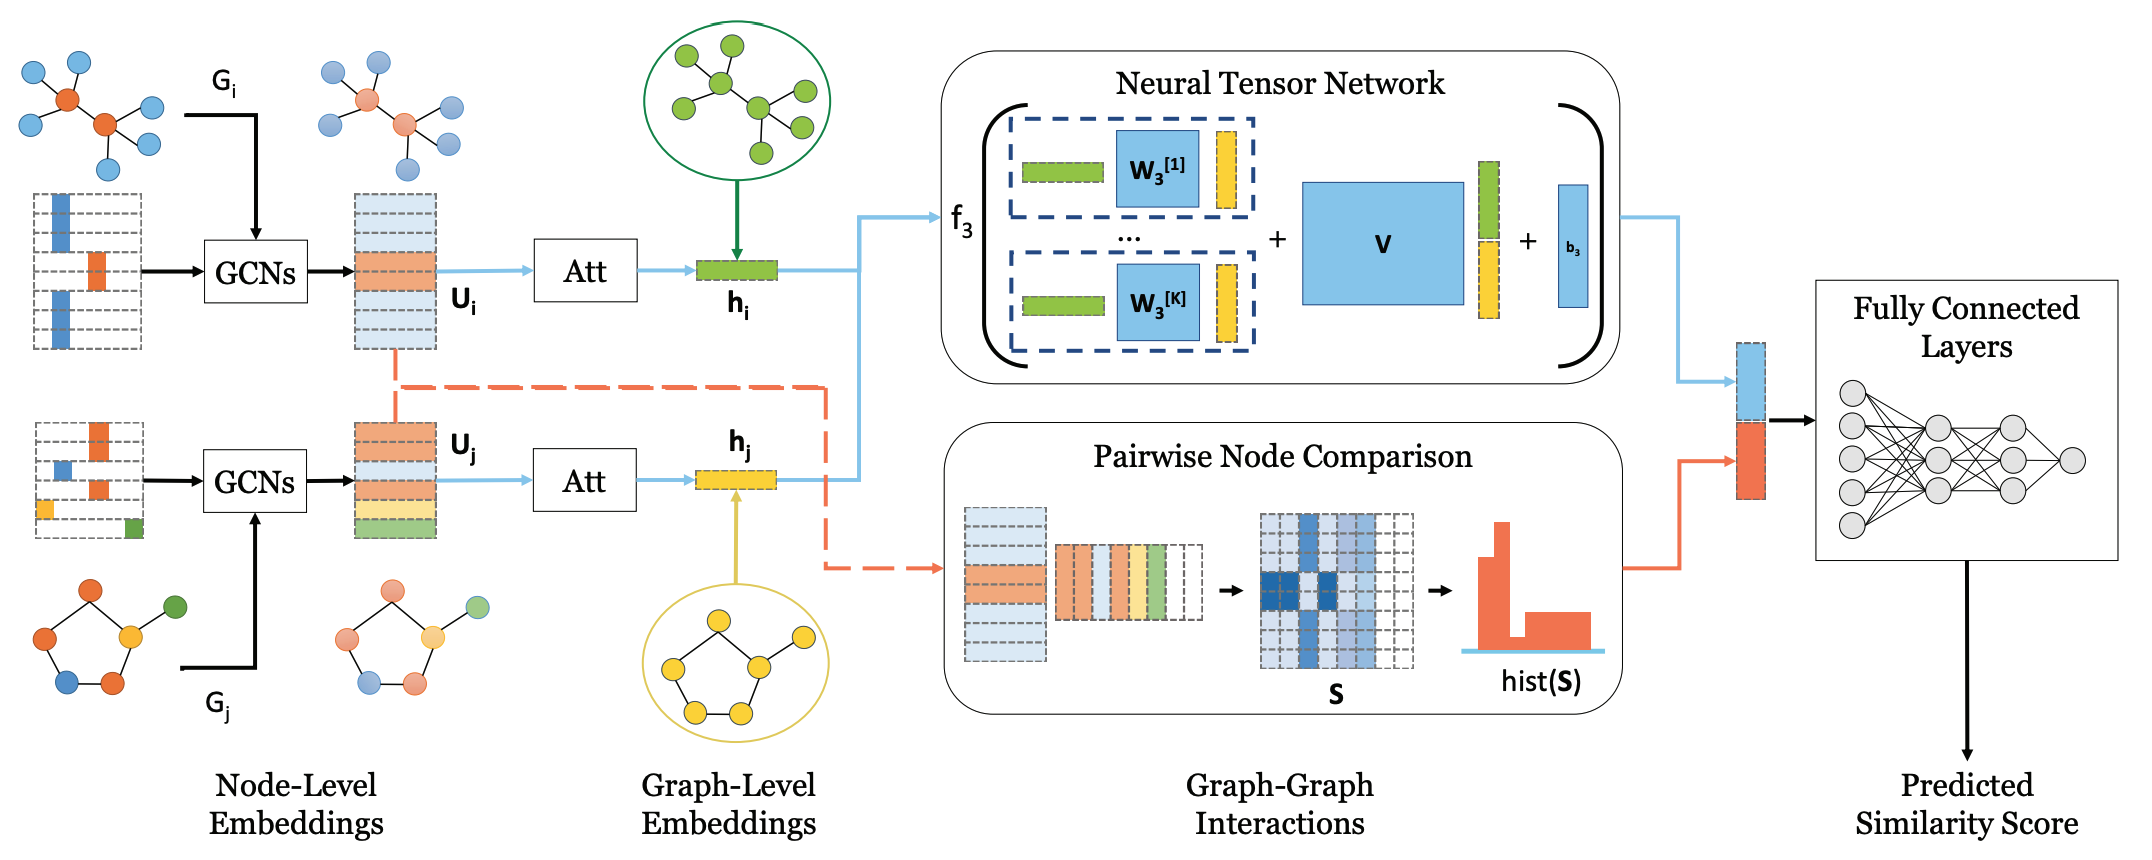
\includegraphics[width=\columnwidth]{Images/Similarity2-1.png}}
Use Neural Tensor Networks (NTN) to model the relation between two graph-level embeddings:
$g(h_i, h_j) = f_3(h_i^TW_3^{[1:k]}h_j + V\begin{bmatrix} h_1 \\ h_j \end{bmatrix} + b_3)$
where $W_3^{[1:k]} \in \mathbb{R}^{D \times D \times K}$ is a weight tensor, $[\cdot]$ is the concatenation operation.
$V \in \mathbb{R}^{K \times 2D}$ is a weight vector, $b_3 \in \mathbb{R}^K$ is a bias vector. $K$ is a hyperparameter controlling the number of interaction scores produced by the model for each graph embedding pair.\\
Feed these similarity scores into a Multi-Layer Perceptron (MLP) to one score $\hat{s}_{ij} \in \mathbb{R}$ to be compared directly in the loss function:
$\mathcal{L} = \frac{1}{|D|} \sum_{(i,j) \in D}(\hat{s}_{i,j} - s(G_i, G_j))^2$
where $D$ is the set of training graph pairs and $s(G_i, G_j)$ is the ground truth similarity.\\
\subsubsection{Pairwise Node Comparison}
To overcome limitations of graph-level embeddings (loss of node feature distribution and graph size) use the node embeddings directly.
Consider graphs $G_i, G_j$ with node embeddings $U_i \in \mathbb{R}^{N_i \times D}, U_j \in \mathbb{R}^{N_j \times D}$ with pairwise interaction scores $S = \sigma(U_iU_j^T)$, zero padding the smaller graph $\implies S \in \mathbb{R}^{N \times N}, N = max(N_i, N_j)$.
To ensure invariance to graph representations, histogram features $hist(S) \in \mathbb{R}^B$ are extracted, where $B$ is a hyperparameter indicating the number of bins. This histogram feature vector is normalized and concatenated with graph level interaction scores and fed to the fully connected layers.

\subsubsection{Evaluation}
Experiments conducted on the following datasets:
\begin{itemize}
    \item \textit{AIDS}: collection of antivirus screen chemical compounds containing 42,687 structures with Hydrogen omitted. Of these 700 were selected, having $\leq$ 10 nodes.
    \item \textit{LINUX}: 48,747 Program Dependence Graphs (PDG) generated from the Linux kernel. Each represents a function, where a node represents a statement and an edge represents the dependency of the statements. (10 nodes or less)
    \item \textit{IMDB}: 15000 ego-networks of actors/actresses, edges determined if they costared in the same film.
\end{itemize}
Shown here are the results for the \textit{LINUX} dataset across the \textit{Spearman's Rank Correlation Coefficient ($\rho$)}, \textit{Kendall's Rank Correlation Coefficient} ($\tau$), and \textit{precision at k} (p@k) – computed by taking the intersection of the top $k$ predicted and ground truth values divided by $k$.
It can be observed that SimGNN exhibits the best performance on \textit{LINUX} across all metrics.
\centerline{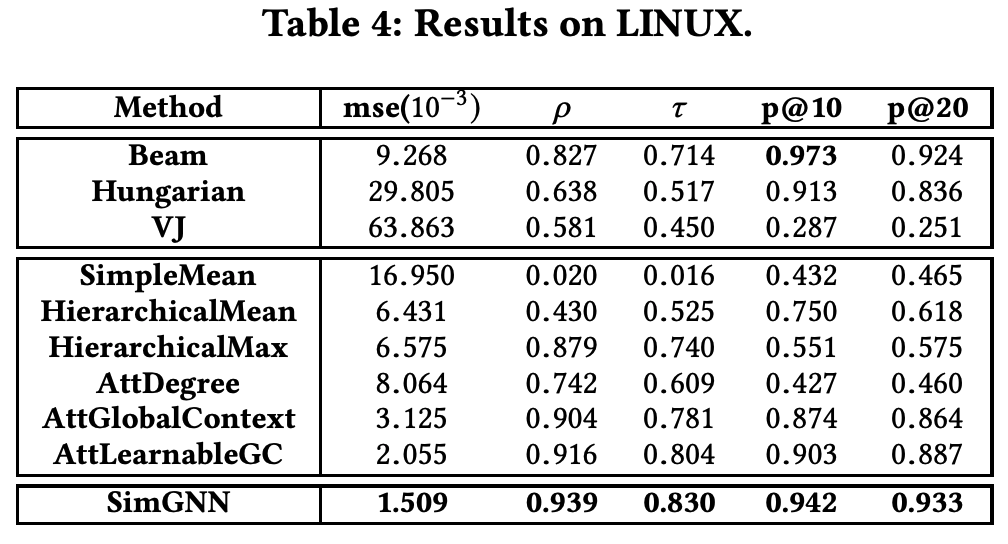
\includegraphics[width=\columnwidth]{Images/Similarity2-2.png}}
\subsubsection{Future Directions}
Work can be done to address the integration of edge features and scalability to larger graphs.

\subsection{Gated Graph Attention Neural Network (GGANN)}
Large scale online programming source code platforms such as Github are rapidly increasing both the number and size of their repositories – necessitating the ability to mine large codebases.
Proposed is the use of Abstract Syntax Trees (AST) to encode the syntactical structure of source code, even attaching data flow edges to encode semantic program meaning in the local scope.
To extend this concept to coarse-grained and global function-call relations, Gated Graph Attention Neural Networks \cite{lu2019program} are proposed. Contributions can be summarized as follows:
\begin{itemize}
    \item Program graph which integrates both data flow and function-call information into AST to characterize syntax and semantics
    \item Improvements made to GGNN model by introducing attention mechanism
\end{itemize}
\centerline{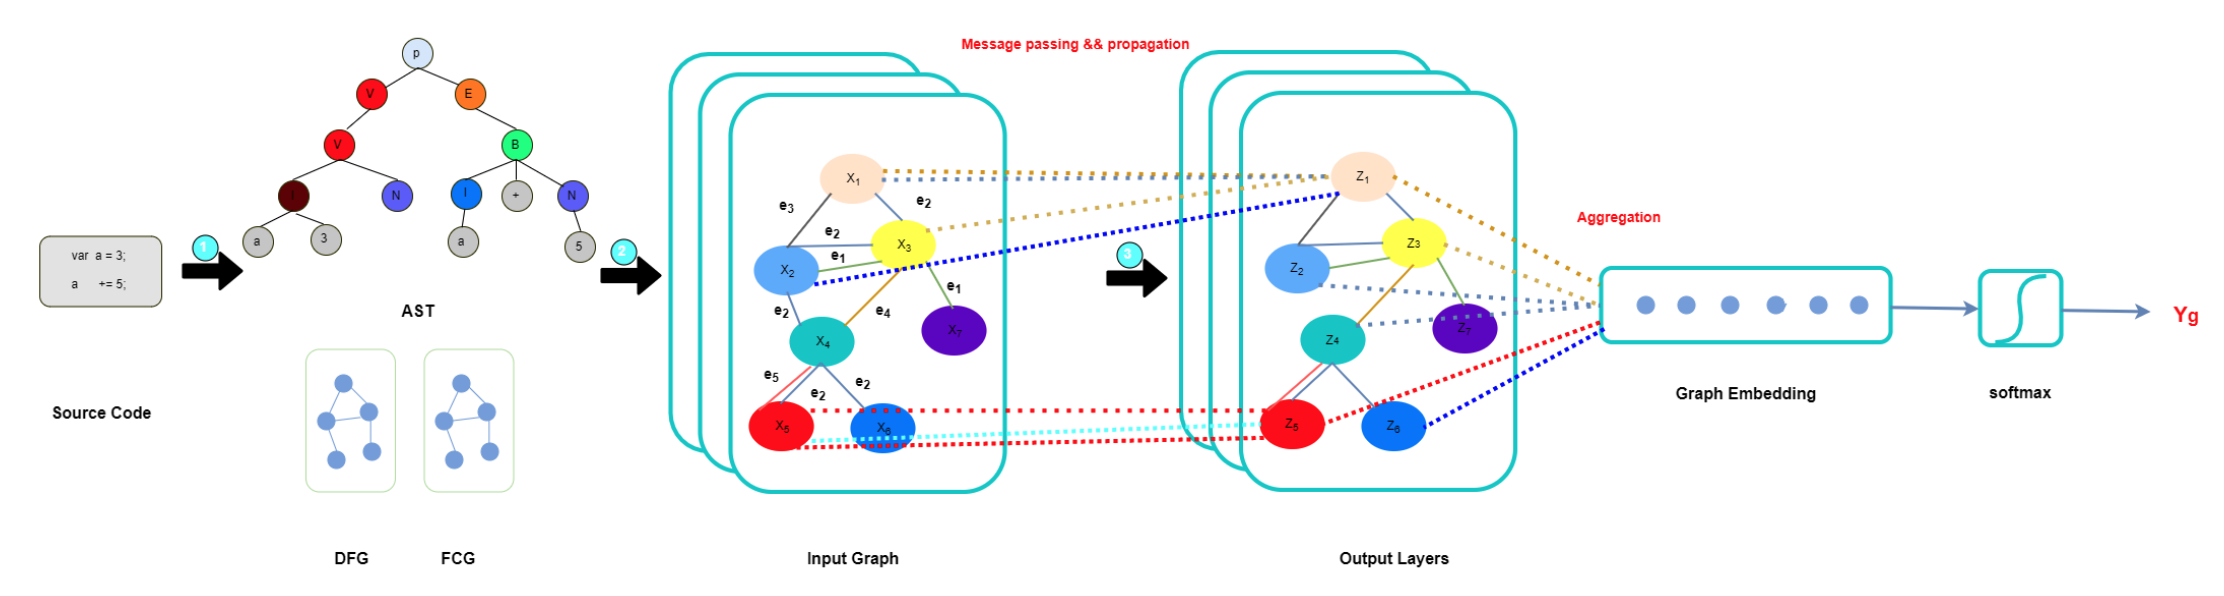
\includegraphics[width=\columnwidth]{Images/Similarity2-4.png}}
Directed graphs are represented as $G = (V,E)$ with edge type set $L_K = {l_1, l_2, \dots, l_k}$, connection matrix $A \in \mathbb{R}^{|V| \times 2|V|}$, where the element $A_{ij}$ is a $d \times d$ matrix, where $d$ represents the feature dimension of a node.
\centerline{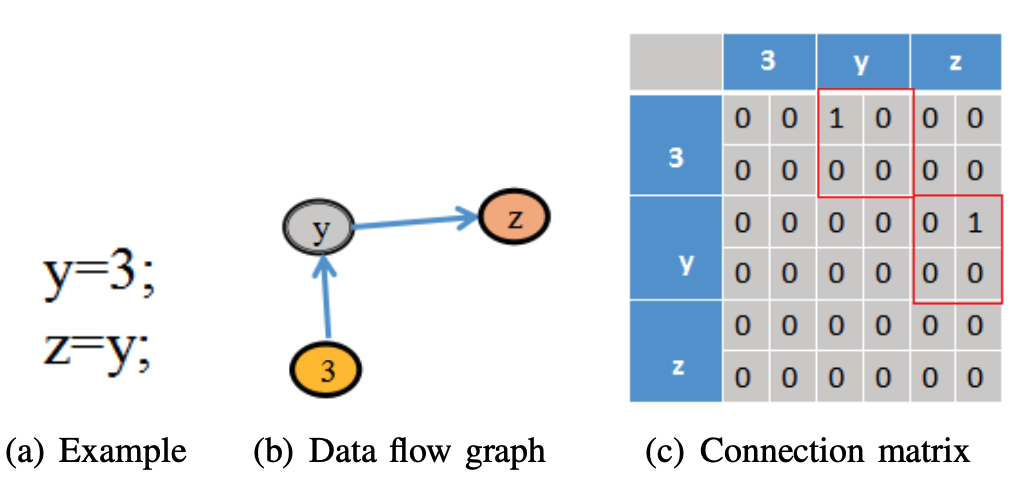
\includegraphics[width=\columnwidth]{Images/Similarity2-3.png}}
Directed graphs are represented as $G = (V,E)$ with edge type set $L_K = {l_1, l_2, \dots, l_k}$, connection matrix $A \in \mathbb{R}^{|V| \times 2|V|}$, where the element $A_{ij}$ is a $d \times d$ matrix, where $d$ represents the feature dimension of a node.
Neighbor state aggregation: $m_i^{(t)} = \sum\limits_{j \in N_i} A_{ij} \cdot h_j^{(t-1)}$ with per node state information: $h_i^{(t)} = GRU(m_t^{(t)}, h_i^{(t-1)})$
\subsubsection{Program Graph Construction}
Program graph construction consists of the construction of the AST, Function Call Graph (FCG), and Data Flow Graph (DFG).
AST is as described in preceding sections. Each node in FCG represents a function, while each edge denotes a function-call relation between two functions.
A node in DFG can be an entity, such as a variable, operator, structure identifier, etc., while an edge represents the data transfer between two entities.
\centerline{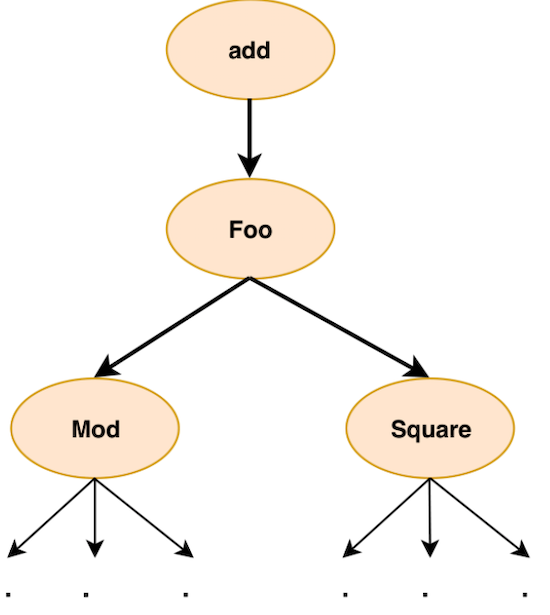
\includegraphics[width=\columnwidth]{Images/Similarity2-5a.png}}
\centerline{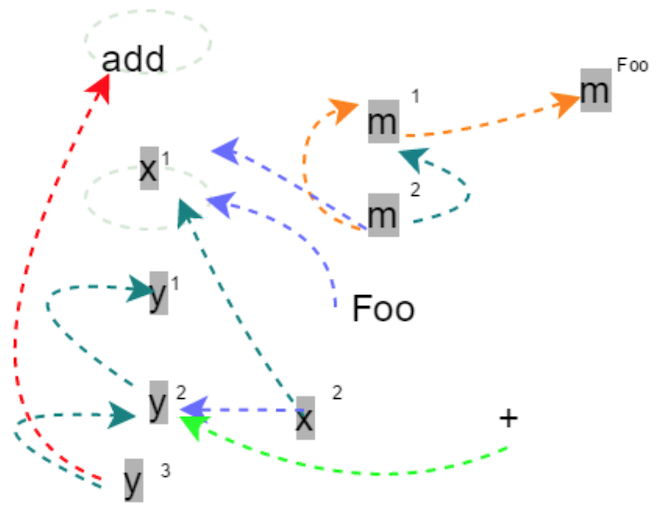
\includegraphics[width=\columnwidth]{Images/Similarity2-5b.png}}
It is desireable to integrate these representations into a new program graph that encapsulates their joint information: called the integrated FDA graph.
\centerline{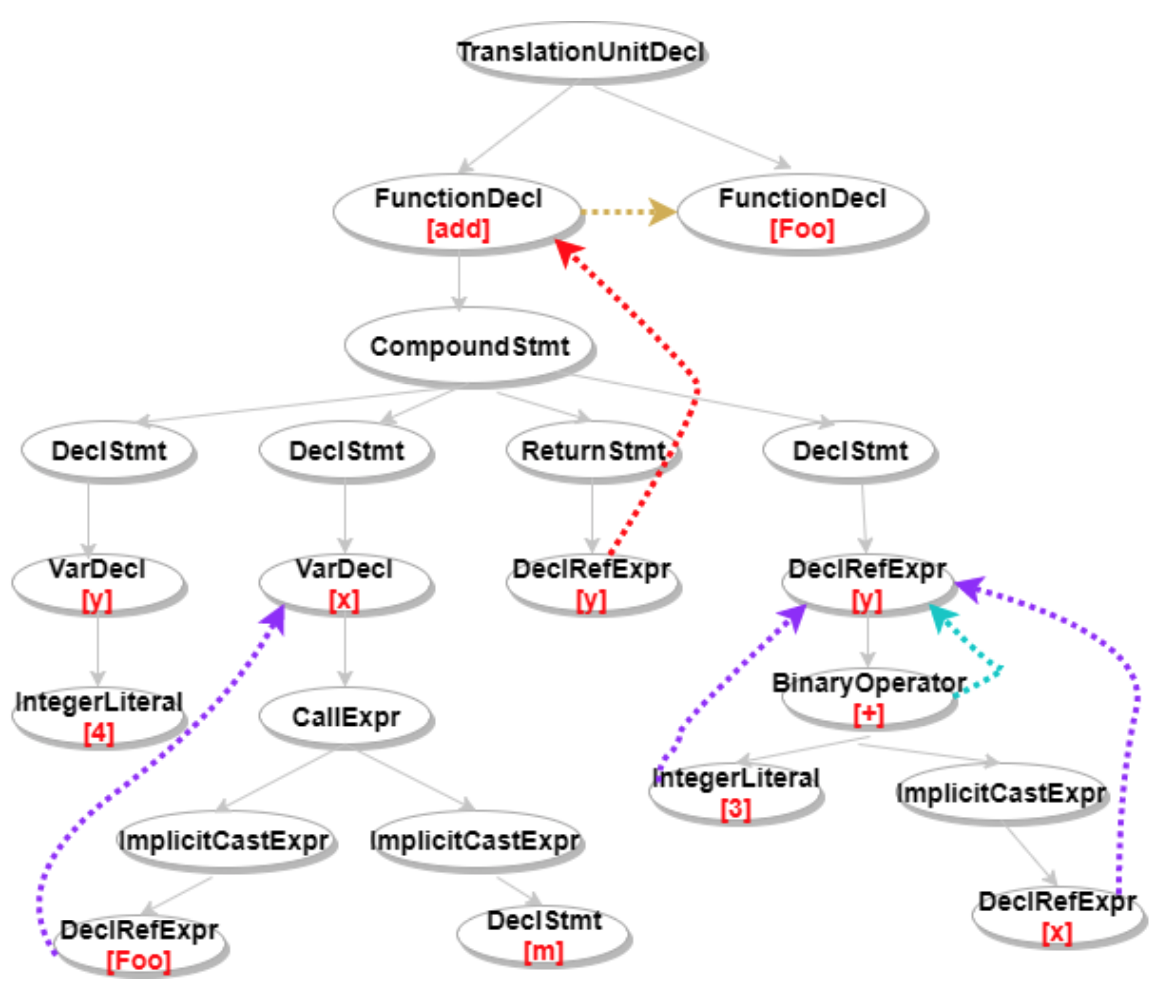
\includegraphics[width=\columnwidth]{Images/Similarity2-6.png}}
In summary, the node information aggregation is as follows:
$m_i^{(t)} = \sum\limits_{j \in N_i}\alpha_{ij} A(h_{ij}^{'(t)}) h_j^{(t-1)}$ with hidden state of directed edge $e_{ij}, \ h'_{ij} = U_e(h_{ij}^{'(t-1)}, h_i^{(t-1)}, h_j^{(t-1)})$ where $U_e$ is a multi-layer neural network.
Propagation matrix $A_{ij}$ can be replaced with a propagation matrix function, $A(h_{ij}') : \mathbb{R}^d \rightarrow \mathbb{R}^{d \times d}$ which learns the propagation matrix dynamically according to the dynamic information of the hidden state, realized by a multilayer neural network.
Information strength $\alpha_{ij} = softmax(a(h_i^{(t-1)}, h_j^{(t-1)}))$, where $a : \mathbb{R}^{d \times d} \rightarrow \mathbb{R}$ is an attention mechanism.
Vector representation for the FDA graph is unknown before calculation of the node's contribution, so it is approximated from the updated hidden state of each node after $T$ iterations of information propagation for sufficiently large $T$.
Embedding vector of the entire FDA graph can be evaluated by computing the weighted sum of node embeddings and an activation.
$h_G = softmax(\sum\limits_{i \in V}f(h_i^{(T)}, x_i) \odot g(h_i^{(T)}))$
\subsubsection{Experimental Evaluation}
Experiments were conducted on the Online Judge (OJ) programming source code files in C++, to be evaluated on classification accuracy, semantic analysis of learned representation, and attention analysis.
\centerline{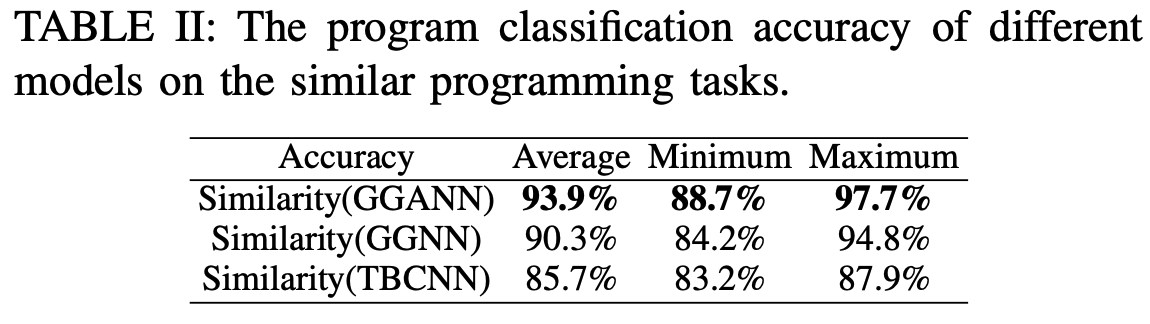
\includegraphics[width=\columnwidth]{Images/Similarity2-7.png}}
Node representations similarity was evaluated using K-means to see if similar nodes clustered into meaningful groups.
\centerline{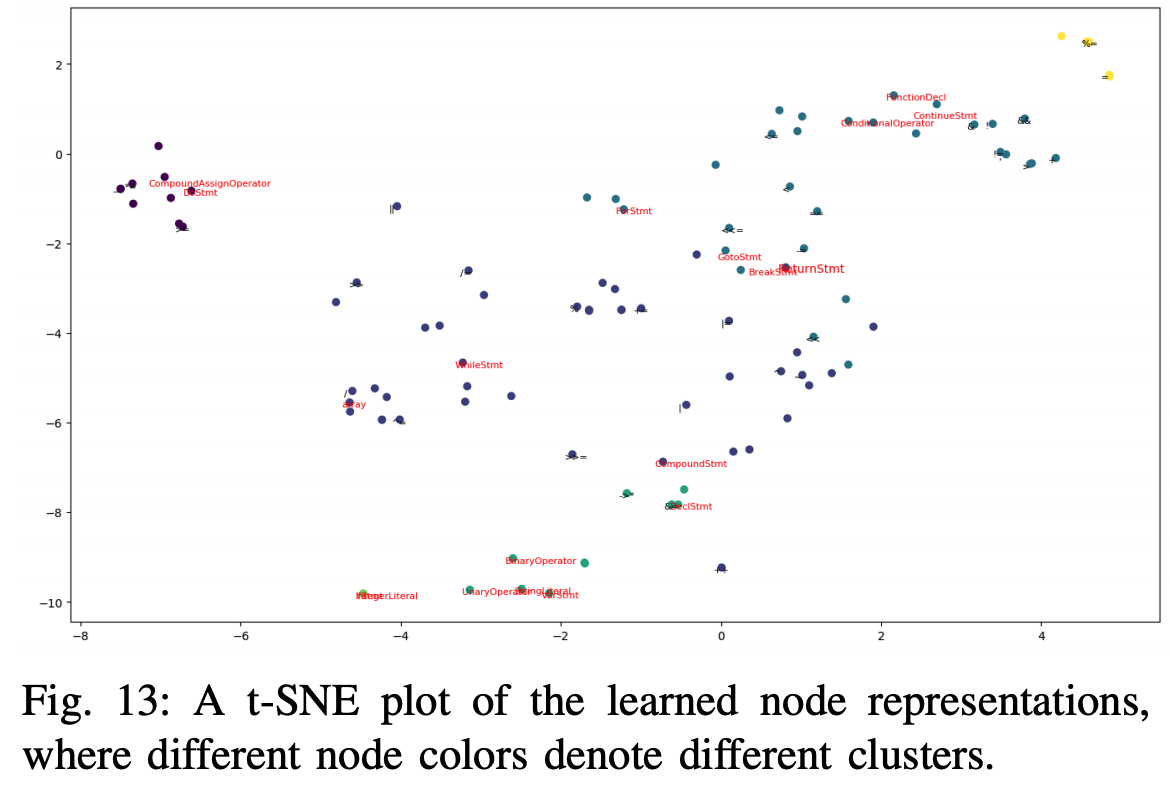
\includegraphics[width=\columnwidth]{Images/Similarity2-8.png}}
The attention mechanism was visualized via a heat map of the node attentions when aggregated to entire graph representations.
\centerline{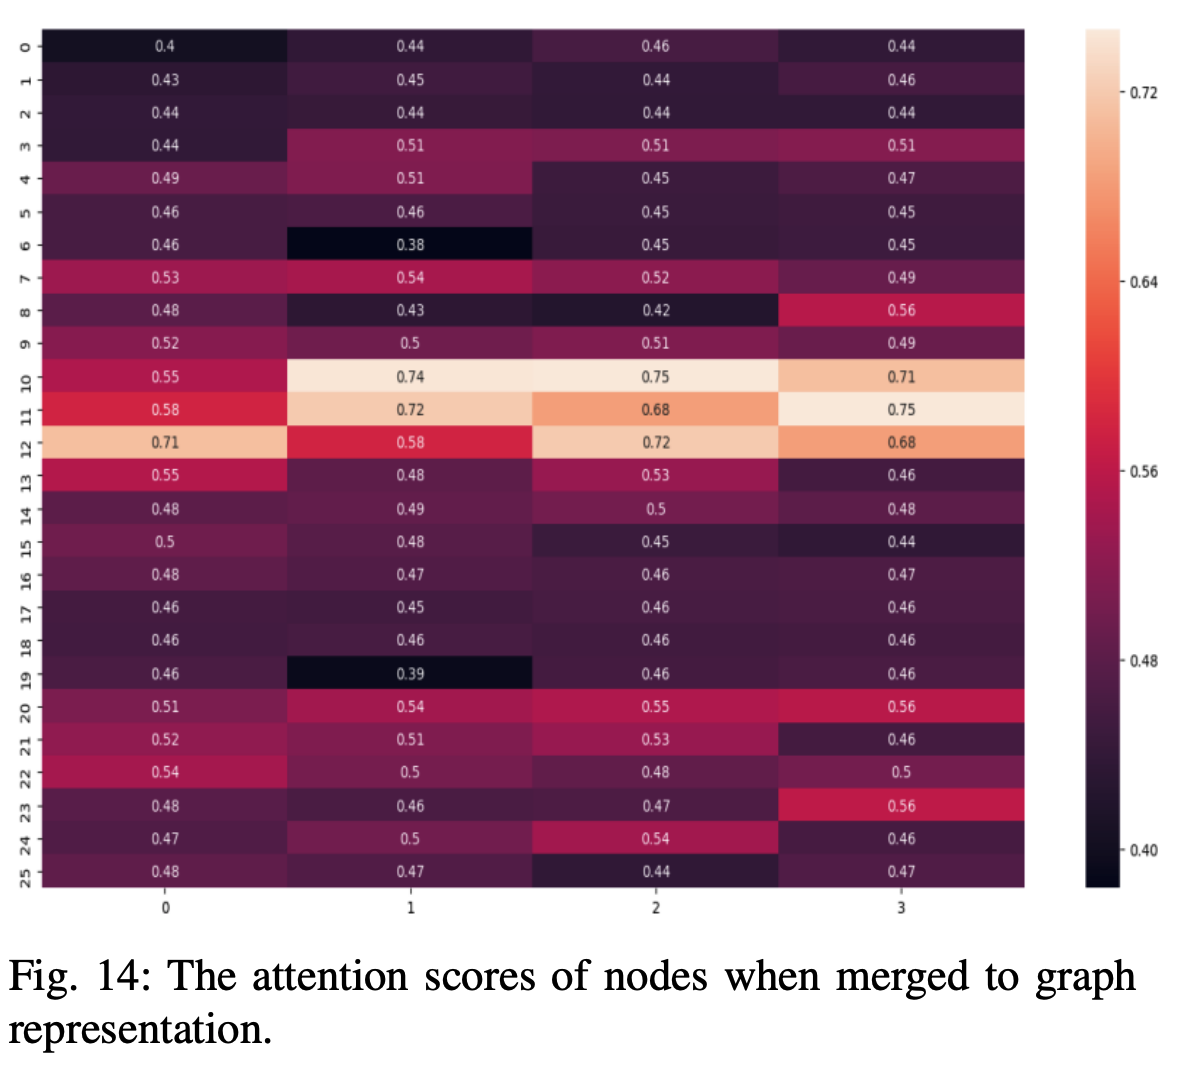
\includegraphics[width=\columnwidth]{Images/Similarity2-9.png}}

\subsection{Graph Matching Networks (GMN)}
Instead of computing graph representations independently for each graph, GMNs compute a similarity score through a cross-graph attention mechanism to associate nodes across graphs and identify differences.
Proposed models are evaluated on three tasks: a synthetic graph edit-distance learning task which captures structural similarity exclusively, and binary function similarity search and mesh retrieval, requiring added semantic similarity.
The contributions of the paper can be summarized as follows:
\begin{itemize}
    \item Demonstration of how GNNs can be used to produce graph embeddings for similarity learning
    \item Proposal of new Graph Matching Networks that compute similarity through cross-graph attention based matching
\end{itemize}
\subsubsection{Graph Embedding Models}
This GNN embedding model consists of an encoder, propagation layers, and an aggregator.\\
\textit{Encoder} maps the node and edge features to initial node and edge vectors through separate\\ MLPs:
$h_i^{(0)} = MLP_{node}(x_i) \  \forall i \in V \\
e_{ij} = MLP_{edge}(x_{ij}), \ \forall (i,j) \in E$\\
\textit{Propagation Layers}\\
$ m_{j \rightarrow i} = f_{message}(h_i^{(t)}, h_j^{(t)}, e_{ij})\\
h_i^{(t+1)} = f_{node}(h_i^{(t)}, \sum_{j:(j,i) \in E} m_{j \rightarrow i})
$ where $f_{message}$ is typically an MLP and $f_{node}$ can either be an MLP or a recurrent neural network core.\\
\textit{Aggregator}\\
After $T$ rounds of propagations, we compute the following graph level representation\\
$h_G = MLP_G(\sum\limits_{i \in V}\sigma(MLP_{gate}(h_i^{(T)}))\odot MLP(h_i^{(T)}))$ which transforms node representations and then uses a weighted sum with gating vectors to aggregate across nodes.
\subsubsection{Graph Matching Networks}
In this network, node updates will take into account aggregated messages at an inter/intra graph perspective, defined as follows
$ m_{j \rightarrow i} = f_{message}(h_i^{(t)}, h_j^{(t)}, e_{ij}), \forall (i,j) \in E_1 \cup E_2\\
  \mu_{j \rightarrow i} = f_{match}(h_i^{(t)}, h_j^{(t)}), \forall i \in V_1, j \in V_2, \text{ or } i \in V_2, j \in V_1\\
  h_i^{(t+1)} = f_{node}(h_i^{(t)}, \sum_j m_{j \rightarrow i}, \sum_{j'}\mu_{j' \rightarrow i})\\
  h_{G_1} = f_G({h_i^{(T)}}_{i \in V_1})\\
  h_{G_1} = f_G({h_i^{(T)}}_{i \in V_2})\\
  s = f_s(h_{G_1}, h_{G_2})\\
$
where $f_s$ is a standard vector space similarity and $f_{match}$ is a function that incorporates an attention based module:
$ a_{j \rightarrow i} = \frac{exp(s_h(h_i^{(t)}, h_j^{(t)}))}{\sum_j exp(s_h(h_i^{(t)}, h_j^{(t)}))}\\
  \mu_{j \rightarrow i} = a_{j \rightarrow i}(h_i^{(t)} - h_j^{(t)})
$ and therefore, \\
$\sum_j \mu_{j \rightarrow i} = \sum_j a_{j \rightarrow i}(h_i^{(t)} - h_j^{(t)}) =  h_i^{(t)} - a_{j \rightarrow i}h_j^{(t)}
$ with attention weights $a_{j \rightarrow i}$ and $\sum_j \mu_{j \rightarrow i}$ intuitively measures the difference between $h_i^{(t)}$ and its closest neighbor in the other graph.
The matching network has the ability to adjust its graph representations based on the compared graph, amplifying disparities if they do not match pairwise.
\subsubsection{Learning}
If similarity learning model is trained pairwise, samples must be labeled as similar and dissimilar, whereas triple training needs only relative similarity between the three samples.
Loss functions are defined respectively:
$L_{pair} = \mathbb{E}_{(G_1, G_2, t)}[max{0.\gamma-t(1-d(G_1,G_2))}]\\
 L_{triplet} = \mathbb{E}_{(G_1, G_2, G_3)}[ma{0,d(G_1,G_2)-d(G_1,G_3) + \gamma}]$
where $t$ is a binary similarity label.
\subsubsection{Evaluation}
Overall results demonstrate that GMns excel on graph similarity learning and consistently outperform other approaches, shown here is the binary function similarity search.
The model was evaluated on data generated by compiling an open source vido processing software \texttt{ffmpeg} using different compilers \texttt{gcc} and \texttt{clang} with various configurations.
\centerline{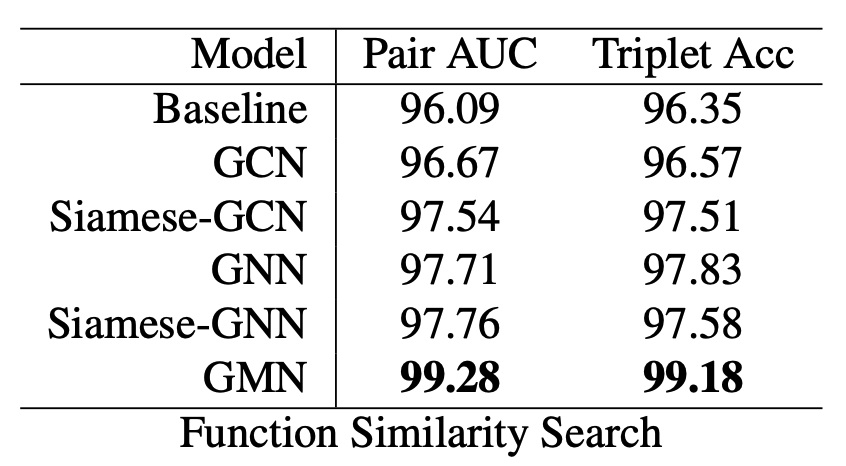
\includegraphics[width=\columnwidth]{Images/Similarity3-1.png}}

\subsection{Neural Code Comprehension \cite{ben2018neural}}
\subsubsection{Introduction}
A novel processing technique to learn code semantics, and apply it to a variety of program analysis tasks – based on an Intermediate Representation (IR), leveraging underlying data- and control-flow of programs.\\
\centerline{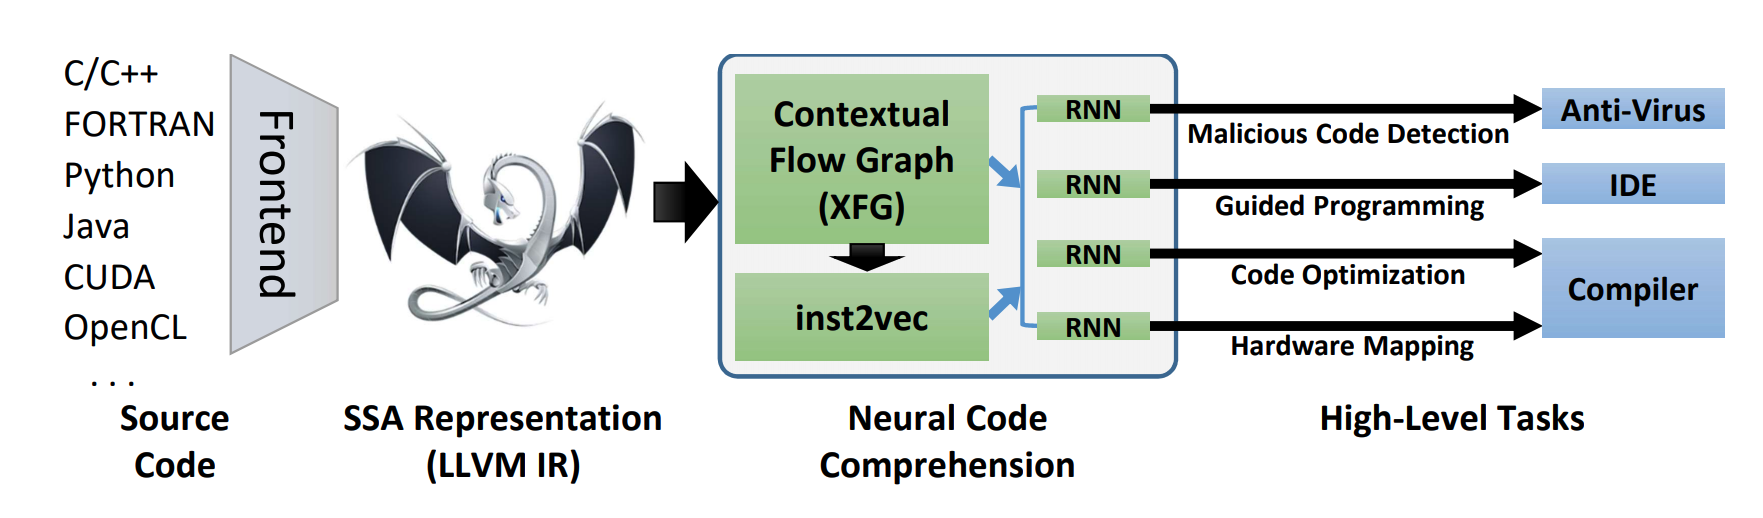
\includegraphics[width=\columnwidth]{Images/Similarity4-1.png}}
\textit{Naturalness Hypothesis: } Software is a form of human communication; software corpora have similar statistical properties to natural language corpora; and these properties can be exploited to build better software engineering tools
This work's contributions are as follows:
\begin{itemize}
    \item Formulation of a robust distributional hypothesis for code, from which a novel distributed representation of code statements based on contextual flow and LLVM IR is drawn.
    \item conteXtual Flow Graphs (XFGs): representation designed for statement embeddings that combine data and control flow
    \item Evaluation using clustering, analogies, semantic tests, and tasks
    \item Using simple LSTM architectures to show leading performance.
\end{itemize}
Robust Distributional Hypothesis of Code can be paraphrased as follows: Statements that occur in the same contexts tend to have similar semantics.
\subsubsection{Contextual Flow Processing}
XFGs are directed multigraphs that provide a notion of context, where nodes (variables or label identifiers) can be connected by more than one edge (data-dependence or execution dependence). 
\textit{XFG Construction}
\begin{enumerate}
    \item Read LLVM IR statements once, storing function names and return statements
    \item Second pass over the statements, adding nodes and edges according to the rule-set:
        \begin{enumerate}[(a)]
            \item Data dependencies within a basic block are connected
            \item Inter-block dependencies are both connected directly and through the label identifier 
            \item Identifiers without a dataflow parent are connected to their root (label or program root)
        \end{enumerate}
\end{enumerate}
\centerline{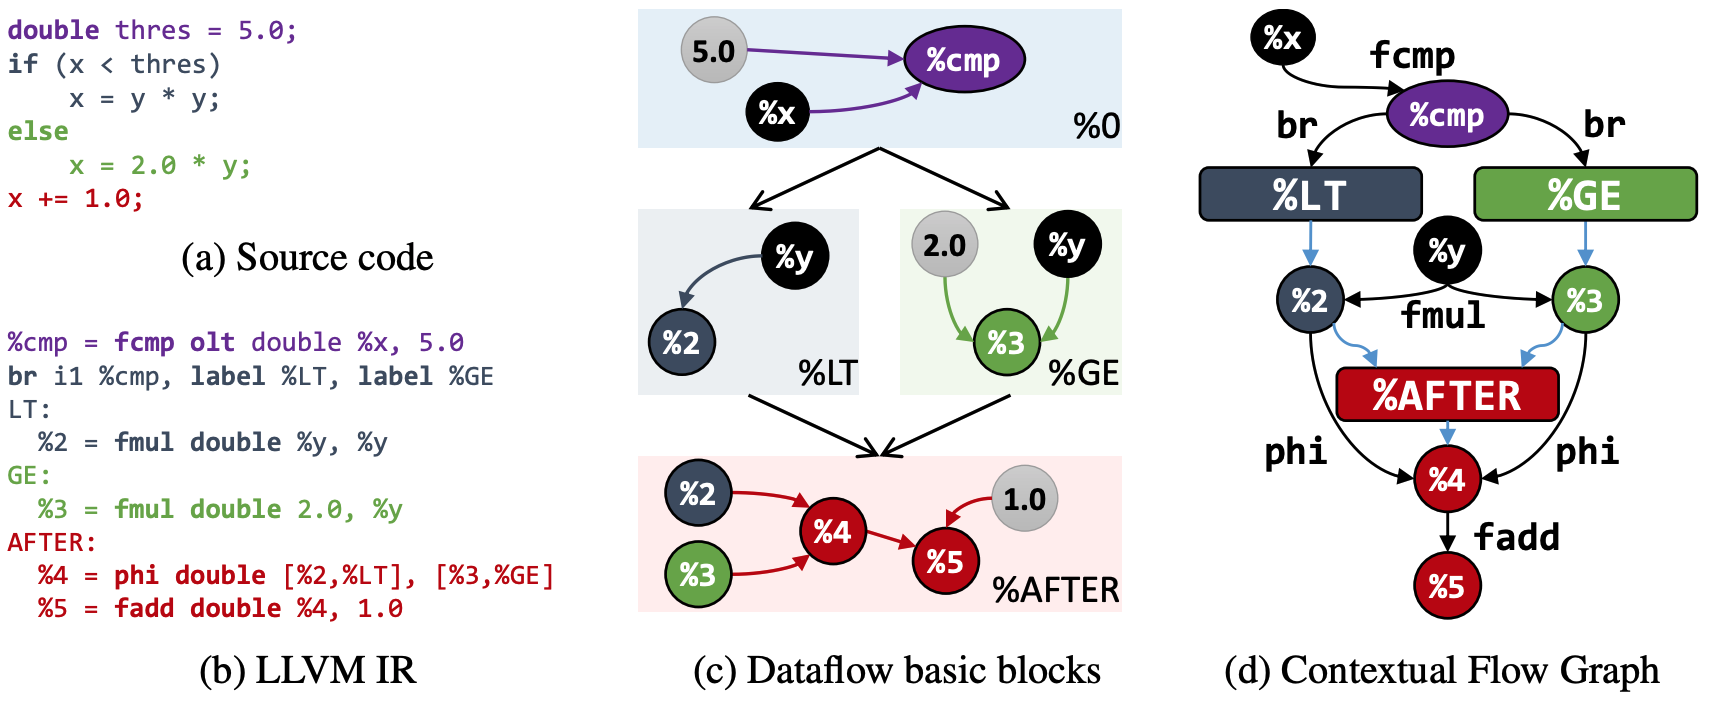
\includegraphics[width=\columnwidth]{Images/Similarity4-2.png}}
\subsubsection{inst2vec: Embedding Statements in Continuous Space}
Desiderata for an embedding space include: (a) statements that are in close proximity should have similar artifacts on a system (i.e. use the same resources); and (b) changing the same attributes (e.g. data type) for different instructions should result in a similar offset in the space.
\centerline{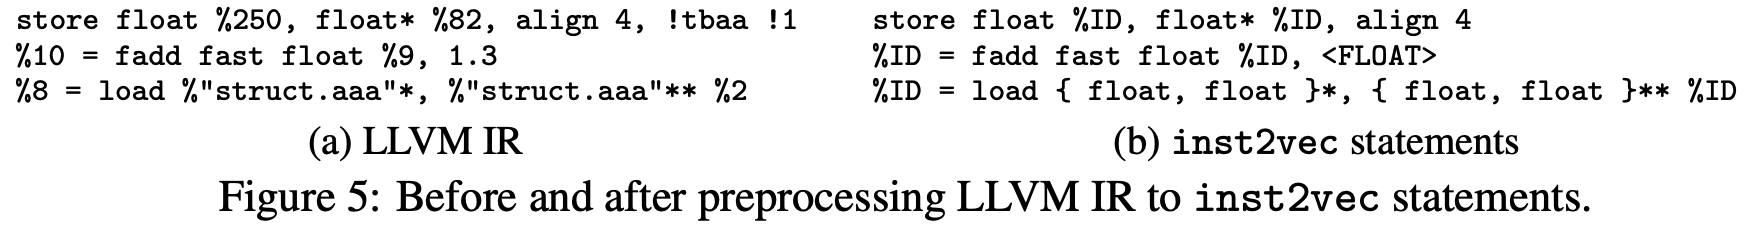
\includegraphics[width=\columnwidth]{Images/Similarity4-3.png}}
\texttt{inst2vec} was generated using corpora from different disciplines, even synthetically generated programs. Given a set of XFGs, neighboring statement pairs up to a certain context size via the skip-gram model are generated.
Pairs are obtained by constructing a dual graph in which statements are nodes, omitting duplicate edges.
\centerline{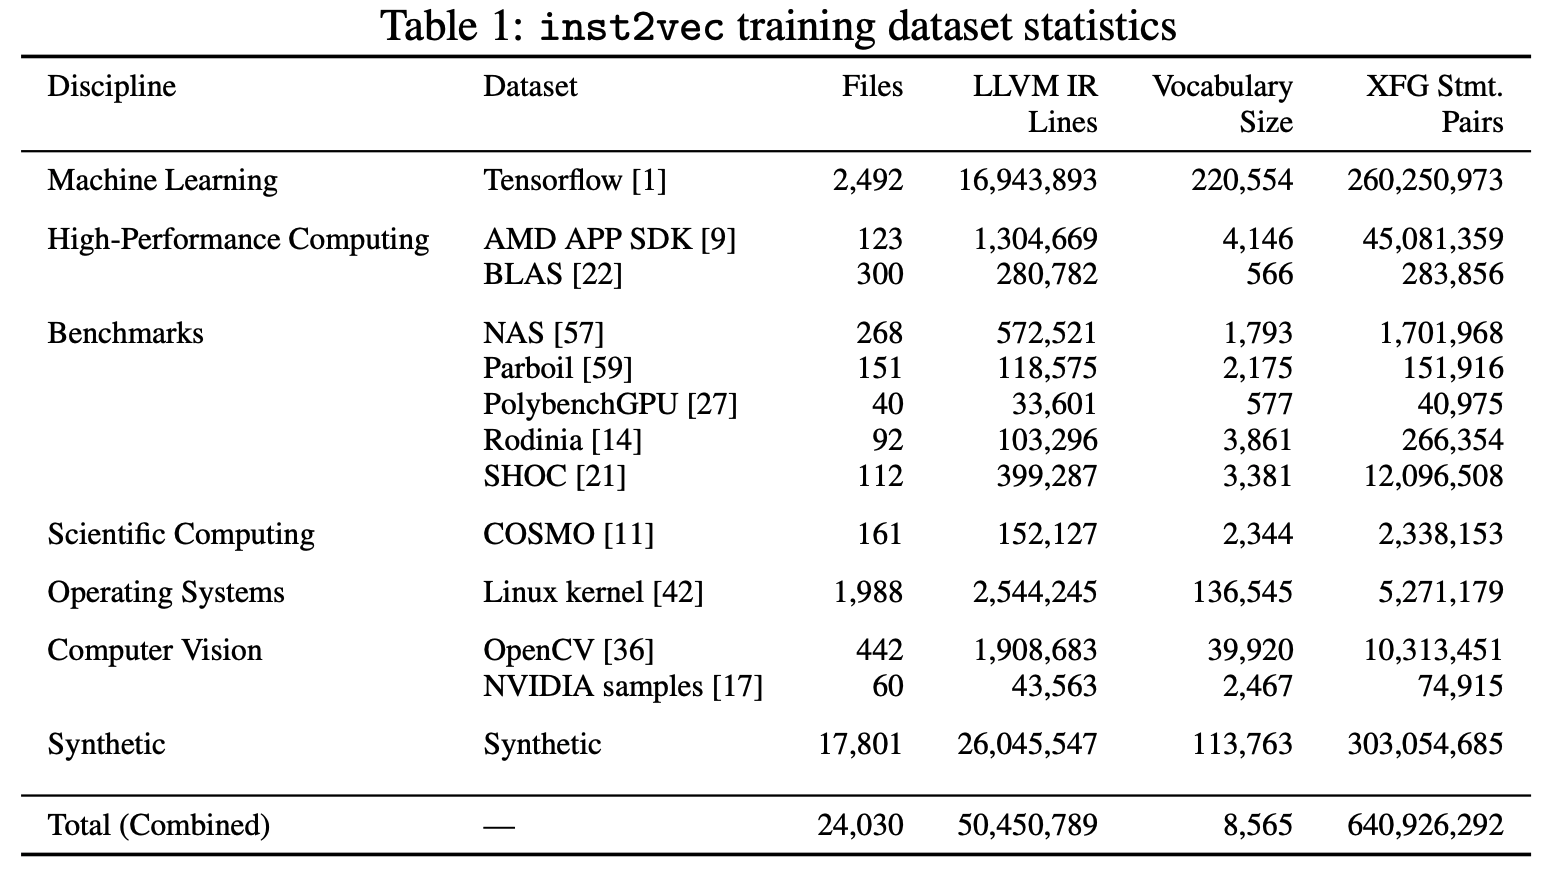
\includegraphics[width=\columnwidth]{Images/Similarity4-4.png}}
\subsubsection{Evaluation}
\centerline{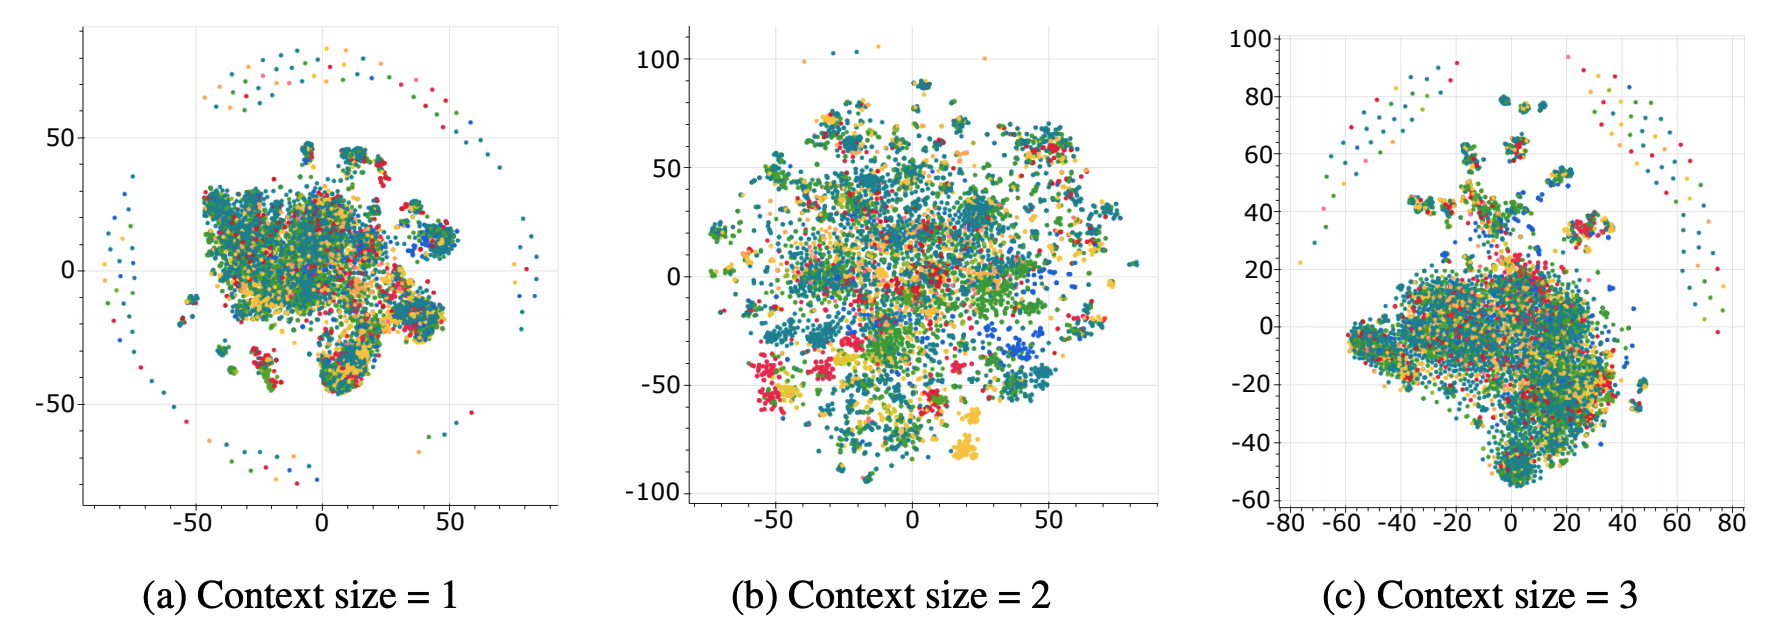
\includegraphics[width=\columnwidth]{Images/Similarity4-5.png}}
Using \texttt{inst2vec} an RNN was constructed that reads source code and outputs a predicted program class on the POJ-104 dataset, collected from the Pedagogical Open Judge System.
\centerline{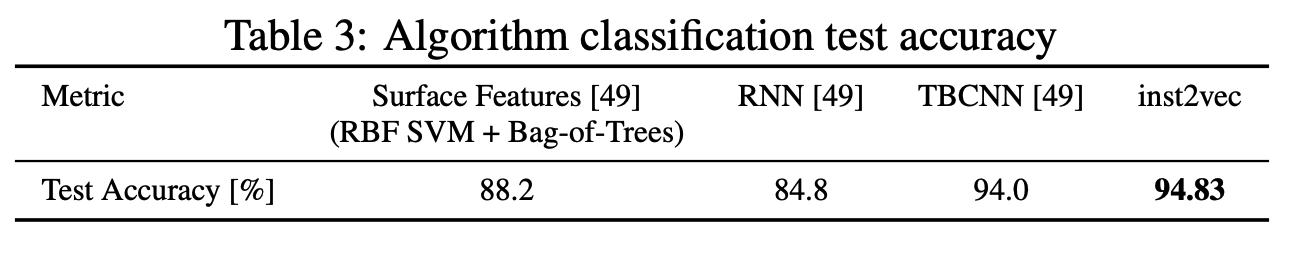
\includegraphics[width=\columnwidth]{Images/Similarity4-6.png}}



\section{Electronic Submission}
\label{submission}

Submission to ICML 2021 will be entirely electronic, via a web site
(not email). Information about the submission process and \LaTeX\ templates
are available on the conference web site at:
\begin{center}
\textbf{\texttt{http://icml.cc/}}
\end{center}

The guidelines below will be enforced for initial submissions and
camera-ready copies. Here is a brief summary:
\begin{itemize}
\item Submissions must be in PDF\@.
\item Submitted papers can be up to eight pages long, not including references, plus unlimited space for references. Accepted papers can be up to nine pages long, not including references, to allow authors to address reviewer comments. Any paper exceeding this length will automatically be rejected. 
\item \textbf{Do not include author information or acknowledgements} in your
    initial submission.
\item Your paper should be in \textbf{10 point Times font}.
\item Make sure your PDF file only uses Type-1 fonts.
\item Place figure captions \emph{under} the figure (and omit titles from inside
    the graphic file itself). Place table captions \emph{over} the table.
\item References must include page numbers whenever possible and be as complete
    as possible. Place multiple citations in chronological order.
\item Do not alter the style template; in particular, do not compress the paper
    format by reducing the vertical spaces.
\item Keep your abstract brief and self-contained, one paragraph and roughly
    4--6 sentences. Gross violations will require correction at the
    camera-ready phase. The title should have content words capitalized.
\end{itemize}

\subsection{Submitting Papers}

\textbf{Paper Deadline:} The deadline for paper submission that is
advertised on the conference website is strict. If your full,
anonymized, submission does not reach us on time, it will not be
considered for publication. 

\textbf{Anonymous Submission:} ICML uses double-blind review: no identifying
author information may appear on the title page or in the paper
itself. Section~\ref{author info} gives further details.

\textbf{Simultaneous Submission:} ICML will not accept any paper which,
at the time of submission, is under review for another conference or
has already been published. This policy also applies to papers that
overlap substantially in technical content with conference papers
under review or previously published. ICML submissions must not be
submitted to other conferences and journals during ICML's review
period.
%Authors may submit to ICML substantially different versions of journal papers
%that are currently under review by the journal, but not yet accepted
%at the time of submission.
Informal publications, such as technical
reports or papers in workshop proceedings which do not appear in
print, do not fall under these restrictions.

\medskip

Authors must provide their manuscripts in \textbf{PDF} format.
Furthermore, please make sure that files contain only embedded Type-1 fonts
(e.g.,~using the program \texttt{pdffonts} in linux or using
File/DocumentProperties/Fonts in Acrobat). Other fonts (like Type-3)
might come from graphics files imported into the document.

Authors using \textbf{Word} must convert their document to PDF\@. Most
of the latest versions of Word have the facility to do this
automatically. Submissions will not be accepted in Word format or any
format other than PDF\@. Really. We're not joking. Don't send Word.

Those who use \textbf{\LaTeX} should avoid including Type-3 fonts.
Those using \texttt{latex} and \texttt{dvips} may need the following
two commands:

{\footnotesize
\begin{verbatim}
dvips -Ppdf -tletter -G0 -o paper.ps paper.dvi
ps2pdf paper.ps
\end{verbatim}}
It is a zero following the ``-G'', which tells dvips to use
the config.pdf file. Newer \TeX\ distributions don't always need this
option.

Using \texttt{pdflatex} rather than \texttt{latex}, often gives better
results. This program avoids the Type-3 font problem, and supports more
advanced features in the \texttt{microtype} package.

\textbf{Graphics files} should be a reasonable size, and included from
an appropriate format. Use vector formats (.eps/.pdf) for plots,
lossless bitmap formats (.png) for raster graphics with sharp lines, and
jpeg for photo-like images.

The style file uses the \texttt{hyperref} package to make clickable
links in documents. If this causes problems for you, add
\texttt{nohyperref} as one of the options to the \texttt{icml2021}
usepackage statement.


\subsection{Submitting Final Camera-Ready Copy}

The final versions of papers accepted for publication should follow the
same format and naming convention as initial submissions, except that
author information (names and affiliations) should be given. See
Section~\ref{final author} for formatting instructions.

The footnote, ``Preliminary work. Under review by the International
Conference on Machine Learning (ICML). Do not distribute.'' must be
modified to ``\textit{Proceedings of the
$\mathit{38}^{th}$ International Conference on Machine Learning},
Online, PMLR 139, 2021.
Copyright 2021 by the author(s).''

For those using the \textbf{\LaTeX} style file, this change (and others) is
handled automatically by simply changing
$\mathtt{\backslash usepackage\{icml2021\}}$ to
$$\mathtt{\backslash usepackage[accepted]\{icml2021\}}$$
Authors using \textbf{Word} must edit the
footnote on the first page of the document themselves.

Camera-ready copies should have the title of the paper as running head
on each page except the first one. The running title consists of a
single line centered above a horizontal rule which is $1$~point thick.
The running head should be centered, bold and in $9$~point type. The
rule should be $10$~points above the main text. For those using the
\textbf{\LaTeX} style file, the original title is automatically set as running
head using the \texttt{fancyhdr} package which is included in the ICML
2021 style file package. In case that the original title exceeds the
size restrictions, a shorter form can be supplied by using

\verb|\icmltitlerunning{...}|

just before $\mathtt{\backslash begin\{document\}}$.
Authors using \textbf{Word} must edit the header of the document themselves.

\section{Format of the Paper}

All submissions must follow the specified format.

\subsection{Dimensions}




The text of the paper should be formatted in two columns, with an
overall width of 6.75~inches, height of 9.0~inches, and 0.25~inches
between the columns. The left margin should be 0.75~inches and the top
margin 1.0~inch (2.54~cm). The right and bottom margins will depend on
whether you print on US letter or A4 paper, but all final versions
must be produced for US letter size.

The paper body should be set in 10~point type with a vertical spacing
of 11~points. Please use Times typeface throughout the text.

\subsection{Title}

The paper title should be set in 14~point bold type and centered
between two horizontal rules that are 1~point thick, with 1.0~inch
between the top rule and the top edge of the page. Capitalize the
first letter of content words and put the rest of the title in lower
case.

\subsection{Author Information for Submission}
\label{author info}

ICML uses double-blind review, so author information must not appear. If
you are using \LaTeX\/ and the \texttt{icml2021.sty} file, use
\verb+\icmlauthor{...}+ to specify authors and \verb+\icmlaffiliation{...}+ to specify affiliations. (Read the TeX code used to produce this document for an example usage.) The author information
will not be printed unless \texttt{accepted} is passed as an argument to the
style file.
Submissions that include the author information will not
be reviewed.

\subsubsection{Self-Citations}

If you are citing published papers for which you are an author, refer
to yourself in the third person. In particular, do not use phrases
that reveal your identity (e.g., ``in previous work \cite{langley00}, we
have shown \ldots'').

Do not anonymize citations in the reference section. The only exception are manuscripts that are
not yet published (e.g., under submission). If you choose to refer to
such unpublished manuscripts \cite{anonymous}, anonymized copies have
to be submitted
as Supplementary Material via CMT\@. However, keep in mind that an ICML
paper should be self contained and should contain sufficient detail
for the reviewers to evaluate the work. In particular, reviewers are
not required to look at the Supplementary Material when writing their
review.

\subsubsection{Camera-Ready Author Information}
\label{final author}

If a paper is accepted, a final camera-ready copy must be prepared.
%
For camera-ready papers, author information should start 0.3~inches below the
bottom rule surrounding the title. The authors' names should appear in 10~point
bold type, in a row, separated by white space, and centered. Author names should
not be broken across lines. Unbolded superscripted numbers, starting 1, should
be used to refer to affiliations.

Affiliations should be numbered in the order of appearance. A single footnote
block of text should be used to list all the affiliations. (Academic
affiliations should list Department, University, City, State/Region, Country.
Similarly for industrial affiliations.)

Each distinct affiliations should be listed once. If an author has multiple
affiliations, multiple superscripts should be placed after the name, separated
by thin spaces. If the authors would like to highlight equal contribution by
multiple first authors, those authors should have an asterisk placed after their
name in superscript, and the term ``\textsuperscript{*}Equal contribution"
should be placed in the footnote block ahead of the list of affiliations. A
list of corresponding authors and their emails (in the format Full Name
\textless{}email@domain.com\textgreater{}) can follow the list of affiliations.
Ideally only one or two names should be listed.

A sample file with author names is included in the ICML2021 style file
package. Turn on the \texttt{[accepted]} option to the stylefile to
see the names rendered. All of the guidelines above are implemented
by the \LaTeX\ style file.

\subsection{Abstract}

The paper abstract should begin in the left column, 0.4~inches below the final
address. The heading `Abstract' should be centered, bold, and in 11~point type.
The abstract body should use 10~point type, with a vertical spacing of
11~points, and should be indented 0.25~inches more than normal on left-hand and
right-hand margins. Insert 0.4~inches of blank space after the body. Keep your
abstract brief and self-contained, limiting it to one paragraph and roughly 4--6
sentences. Gross violations will require correction at the camera-ready phase.

\subsection{Partitioning the Text}

You should organize your paper into sections and paragraphs to help
readers place a structure on the material and understand its
contributions.

\subsubsection{Sections and Subsections}

Section headings should be numbered, flush left, and set in 11~pt bold
type with the content words capitalized. Leave 0.25~inches of space
before the heading and 0.15~inches after the heading.

Similarly, subsection headings should be numbered, flush left, and set
in 10~pt bold type with the content words capitalized. Leave
0.2~inches of space before the heading and 0.13~inches afterward.

Finally, subsubsection headings should be numbered, flush left, and
set in 10~pt small caps with the content words capitalized. Leave
0.18~inches of space before the heading and 0.1~inches after the
heading.

Please use no more than three levels of headings.

\subsubsection{Paragraphs and Footnotes}

Within each section or subsection, you should further partition the
paper into paragraphs. Do not indent the first line of a given
paragraph, but insert a blank line between succeeding ones.

You can use footnotes\footnote{Footnotes
should be complete sentences.} to provide readers with additional
information about a topic without interrupting the flow of the paper.
Indicate footnotes with a number in the text where the point is most
relevant. Place the footnote in 9~point type at the bottom of the
column in which it appears. Precede the first footnote in a column
with a horizontal rule of 0.8~inches.\footnote{Multiple footnotes can
appear in each column, in the same order as they appear in the text,
but spread them across columns and pages if possible.}

\begin{figure}[ht]
\vskip 0.2in
\begin{center}
\centerline{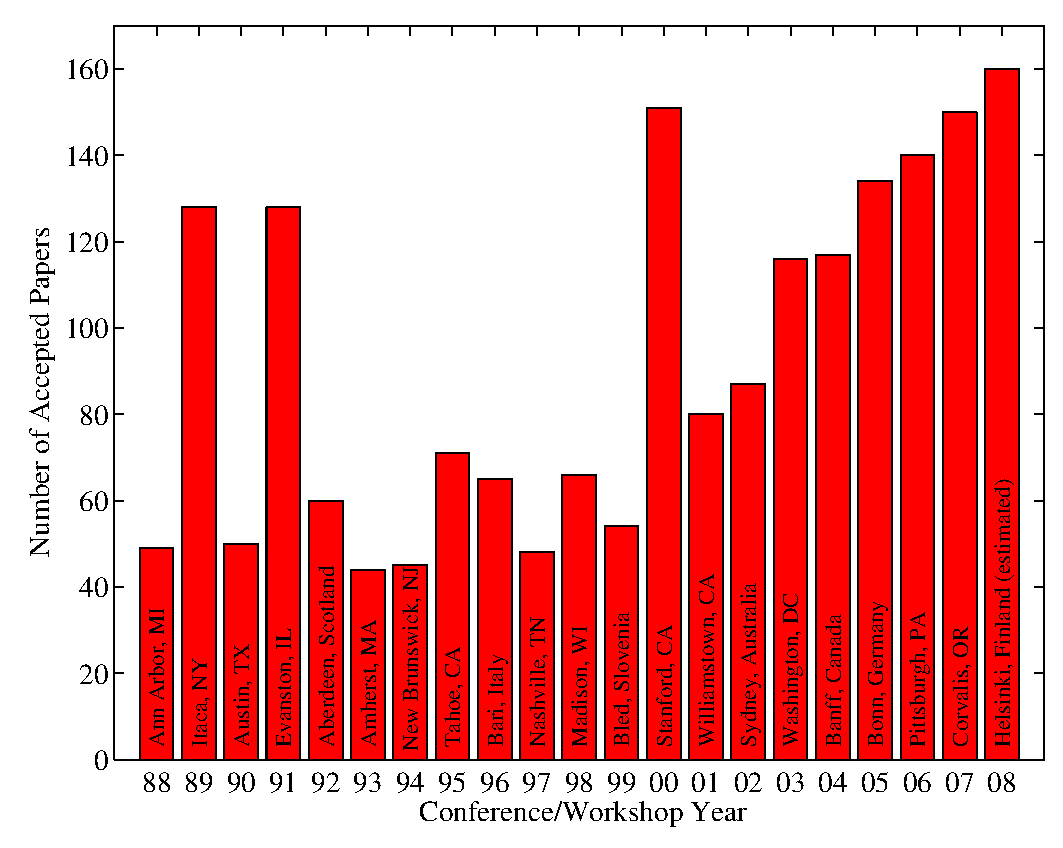
\includegraphics[width=\columnwidth]{icml_numpapers}}
\caption{Historical locations and number of accepted papers for International
Machine Learning Conferences (ICML 1993 -- ICML 2008) and International
Workshops on Machine Learning (ML 1988 -- ML 1992). At the time this figure was
produced, the number of accepted papers for ICML 2008 was unknown and instead
estimated.}
\label{icml-historical}
\end{center}
\vskip -0.2in
\end{figure}

\subsection{Figures}

You may want to include figures in the paper to illustrate
your approach and results. Such artwork should be centered,
legible, and separated from the text. Lines should be dark and at
least 0.5~points thick for purposes of reproduction, and text should
not appear on a gray background.

Label all distinct components of each figure. If the figure takes the
form of a graph, then give a name for each axis and include a legend
that briefly describes each curve. Do not include a title inside the
figure; instead, the caption should serve this function.

Number figures sequentially, placing the figure number and caption
\emph{after} the graphics, with at least 0.1~inches of space before
the caption and 0.1~inches after it, as in
Figure~\ref{icml-historical}. The figure caption should be set in
9~point type and centered unless it runs two or more lines, in which
case it should be flush left. You may float figures to the top or
bottom of a column, and you may set wide figures across both columns
(use the environment \texttt{figure*} in \LaTeX). Always place
two-column figures at the top or bottom of the page.

\subsection{Algorithms}

If you are using \LaTeX, please use the ``algorithm'' and ``algorithmic''
environments to format pseudocode. These require
the corresponding stylefiles, algorithm.sty and
algorithmic.sty, which are supplied with this package.
Algorithm~\ref{alg:example} shows an example.

\begin{algorithm}[tb]
   \caption{Bubble Sort}
   \label{alg:example}
\begin{algorithmic}
   \STATE {\bfseries Input:} data $x_i$, size $m$
   \REPEAT
   \STATE Initialize $noChange = true$.
   \FOR{$i=1$ {\bfseries to} $m-1$}
   \IF{$x_i > x_{i+1}$}
   \STATE Swap $x_i$ and $x_{i+1}$
   \STATE $noChange = false$
   \ENDIF
   \ENDFOR
   \UNTIL{$noChange$ is $true$}
\end{algorithmic}
\end{algorithm}

\subsection{Tables}

You may also want to include tables that summarize material. Like
figures, these should be centered, legible, and numbered consecutively.
However, place the title \emph{above} the table with at least
0.1~inches of space before the title and the same after it, as in
Table~\ref{sample-table}. The table title should be set in 9~point
type and centered unless it runs two or more lines, in which case it
should be flush left.

% Note use of \abovespace and \belowspace to get reasonable spacing
% above and below tabular lines.

\begin{table}[t]
\caption{Classification accuracies for naive Bayes and flexible
Bayes on various data sets.}
\label{sample-table}
\vskip 0.15in
\begin{center}
\begin{small}
\begin{sc}
\begin{tabular}{lcccr}
\toprule
Data set & Naive & Flexible & Better? \\
\midrule
Breast    & 95.9$\pm$ 0.2& 96.7$\pm$ 0.2& $\surd$ \\
Cleveland & 83.3$\pm$ 0.6& 80.0$\pm$ 0.6& $\times$\\
Glass2    & 61.9$\pm$ 1.4& 83.8$\pm$ 0.7& $\surd$ \\
Credit    & 74.8$\pm$ 0.5& 78.3$\pm$ 0.6&         \\
Horse     & 73.3$\pm$ 0.9& 69.7$\pm$ 1.0& $\times$\\
Meta      & 67.1$\pm$ 0.6& 76.5$\pm$ 0.5& $\surd$ \\
Pima      & 75.1$\pm$ 0.6& 73.9$\pm$ 0.5&         \\
Vehicle   & 44.9$\pm$ 0.6& 61.5$\pm$ 0.4& $\surd$ \\
\bottomrule
\end{tabular}
\end{sc}
\end{small}
\end{center}
\vskip -0.1in
\end{table}

Tables contain textual material, whereas figures contain graphical material.
Specify the contents of each row and column in the table's topmost
row. Again, you may float tables to a column's top or bottom, and set
wide tables across both columns. Place two-column tables at the
top or bottom of the page.

\subsection{Citations and References}

Please use APA reference format regardless of your formatter
or word processor. If you rely on the \LaTeX\/ bibliographic
facility, use \texttt{natbib.sty} and \texttt{icml2021.bst}
included in the style-file package to obtain this format.

Citations within the text should include the authors' last names and
year. If the authors' names are included in the sentence, place only
the year in parentheses, for example when referencing Arthur Samuel's
pioneering work \yrcite{Samuel59}. Otherwise place the entire
reference in parentheses with the authors and year separated by a
comma \cite{Samuel59}. List multiple references separated by
semicolons \cite{kearns89,Samuel59,mitchell80}. Use the `et~al.'
construct only for citations with three or more authors or after
listing all authors to a publication in an earlier reference \cite{MachineLearningI}.

Authors should cite their own work in the third person
in the initial version of their paper submitted for blind review.
Please refer to Section~\ref{author info} for detailed instructions on how to
cite your own papers.

Use an unnumbered first-level section heading for the references, and use a
hanging indent style, with the first line of the reference flush against the
left margin and subsequent lines indented by 10 points. The references at the
end of this document give examples for journal articles \cite{Samuel59},
conference publications \cite{langley00}, book chapters \cite{Newell81}, books
\cite{DudaHart2nd}, edited volumes \cite{MachineLearningI}, technical reports
\cite{mitchell80}, and dissertations \cite{kearns89}.

Alphabetize references by the surnames of the first authors, with
single author entries preceding multiple author entries. Order
references for the same authors by year of publication, with the
earliest first. Make sure that each reference includes all relevant
information (e.g., page numbers).

Please put some effort into making references complete, presentable, and
consistent. If using bibtex, please protect capital letters of names and
abbreviations in titles, for example, use \{B\}ayesian or \{L\}ipschitz
in your .bib file.

\section*{Software and Data}

If a paper is accepted, we strongly encourage the publication of software and data with the
camera-ready version of the paper whenever appropriate. This can be
done by including a URL in the camera-ready copy. However, \textbf{do not}
include URLs that reveal your institution or identity in your
submission for review. Instead, provide an anonymous URL or upload
the material as ``Supplementary Material'' into the CMT reviewing
system. Note that reviewers are not required to look at this material
when writing their review.

% Acknowledgements should only appear in the accepted version.
\section*{Acknowledgements}

\textbf{Do not} include acknowledgements in the initial version of
the paper submitted for blind review.

If a paper is accepted, the final camera-ready version can (and
probably should) include acknowledgements. In this case, please
place such acknowledgements in an unnumbered section at the
end of the paper. Typically, this will include thanks to reviewers
who gave useful comments, to colleagues who contributed to the ideas,
and to funding agencies and corporate sponsors that provided financial
support.


% In the unusual situation where you want a paper to appear in the
% references without citing it in the main text, use \nocite
\nocite{langley00}

\bibliography{main}
\bibliographystyle{icml2021}


%%%%%%%%%%%%%%%%%%%%%%%%%%%%%%%%%%%%%%%%%%%%%%%%%%%%%%%%%%%%%%%%%%%%%%%%%%%%%%%
%%%%%%%%%%%%%%%%%%%%%%%%%%%%%%%%%%%%%%%%%%%%%%%%%%%%%%%%%%%%%%%%%%%%%%%%%%%%%%%
% DELETE THIS PART. DO NOT PLACE CONTENT AFTER THE REFERENCES!
%%%%%%%%%%%%%%%%%%%%%%%%%%%%%%%%%%%%%%%%%%%%%%%%%%%%%%%%%%%%%%%%%%%%%%%%%%%%%%%
%%%%%%%%%%%%%%%%%%%%%%%%%%%%%%%%%%%%%%%%%%%%%%%%%%%%%%%%%%%%%%%%%%%%%%%%%%%%%%%
\appendix
\section{Do \emph{not} have an appendix here}

\textbf{\emph{Do not put content after the references.}}
%
Put anything that you might normally include after the references in a separate
supplementary file.

We recommend that you build supplementary material in a separate document.
If you must create one PDF and cut it up, please be careful to use a tool that
doesn't alter the margins, and that doesn't aggressively rewrite the PDF file.
pdftk usually works fine. 

\textbf{Please do not use Apple's preview to cut off supplementary material.} In
previous years it has altered margins, and created headaches at the camera-ready
stage. 
%%%%%%%%%%%%%%%%%%%%%%%%%%%%%%%%%%%%%%%%%%%%%%%%%%%%%%%%%%%%%%%%%%%%%%%%%%%%%%%
%%%%%%%%%%%%%%%%%%%%%%%%%%%%%%%%%%%%%%%%%%%%%%%%%%%%%%%%%%%%%%%%%%%%%%%%%%%%%%%


\end{document}


% This document was modified from the file originally made available by
% Pat Langley and Andrea Danyluk for ICML-2K. This version was created
% by Iain Murray in 2018, and modified by Alexandre Bouchard in
% 2019 and 2021. Previous contributors include Dan Roy, Lise Getoor and Tobias
% Scheffer, which was slightly modified from the 2010 version by
% Thorsten Joachims & Johannes Fuernkranz, slightly modified from the
% 2009 version by Kiri Wagstaff and Sam Roweis's 2008 version, which is
% slightly modified from Prasad Tadepalli's 2007 version which is a
% lightly changed version of the previous year's version by Andrew
% Moore, which was in turn edited from those of Kristian Kersting and
% Codrina Lauth. Alex Smola contributed to the algorithmic style files.
